%You can leave alone everything before Line 79.
\documentclass{article}
\usepackage{url,amsfonts, amsmath, amssymb, amsthm,color, enumerate, verbatim}
% Page layout
\setlength{\textheight}{8.75in}
\setlength{\columnsep}{2.0pc}
\setlength{\textwidth}{6.5in}
\setlength{\topmargin}{0in}
\setlength{\headheight}{0.0in}
\setlength{\headsep}{0.0in}
\setlength{\oddsidemargin}{0in}
\setlength{\evensidemargin}{0in}
\setlength{\parindent}{1pc}
\newcommand{\shortbar}{\begin{center}\rule{5ex}{0.1pt}\end{center}}
%\renewcommand{\baselinestretch}{1.1}
% Macros for course info
\newcommand{\courseNumber}{ME 552}
\newcommand{\courseTitle}{Mechatronics}
\newcommand{\semester}{Fall 2012}
\newcommand{\xxx}[1]{\textcolor{red}{#1}}
% Theorem-like structures are numbered within SECTION units
\theoremstyle{plain}
\newtheorem{theorem}{Theorem}[section]
\newtheorem{lemma}[theorem]{Lemma}
\newtheorem{corollary}[theorem]{Corollary}
\newtheorem{proposition}[theorem]{Proposition}
\newtheorem{statement}[theorem]{Statement}
\newtheorem{conjecture}[theorem]{Conjecture}
\newtheorem{fact}{Fact}
%definition style
\theoremstyle{definition}
\newtheorem{definition}[theorem]{Definition}
\newtheorem{example}{Example}
\newtheorem{problem}[theorem]{Problem}
\newtheorem{exercise}{Exercise}
\newtheorem{algorithm}{Algorithm}
%remark style
\theoremstyle{remark}
\newtheorem{remark}[theorem]{Remark}
\newtheorem{reduction}[theorem]{Reduction}
%\newtheorem{question}[theorem]{Question}
\newtheorem{question}{Question}
%\newtheorem{claim}[theorem]{Claim}
%
% Proof-making commands and environments
\newcommand{\beginproof}{\medskip\noindent{\bf Proof.~}}
\newcommand{\beginproofof}[1]{\medskip\noindent{\bf Proof of #1.~}}
\newcommand{\finishproof}{\hspace{0.2ex}\rule{1ex}{1ex}}
\def\therefore{\boldsymbol{\text{ }
\leavevmode
\lower0.4ex\hbox{$\cdot$}
\kern-.5em\raise0.7ex\hbox{$\cdot$}
\kern-0.55em\lower0.4ex\hbox{$\cdot$}
\thinspace\text{ }}}

\newenvironment{solution}[1]{\medskip\noindent{\bf Problem #1.~}}{\shortbar}

%====header======
\newcommand{\solutions}[4]{
%\renewcommand{\thetheorem}{{#2}.\arabic{theorem}}
\vspace{-2ex}
\begin{center}
{\small  \courseNumber, \courseTitle
\hfill {\Large \bf {#1} }\\
\semester, University of Michigan, Ann Arbor \hfill
{\em Date: #3}}\\
\vspace{-1ex}
\hrulefill\\
\vspace{4ex}
{\LARGE Lab Assignment #2}\\
\vspace{2ex}
\end{center}
\begin{trivlist}
\item \textsc{Team members:\\} {#4}
\end{trivlist}
\noindent
\shortbar
\vspace{3ex}
}
% math macros
\newcommand{\defeq}{\stackrel{\textrm{def}}{=}}
\newcommand{\Prob}{\textrm{Prob}}
%==
\usepackage{graphicx}
\usepackage{xfrac}
\usepackage{amsmath}
\providecommand{\e}[1]{\ensuremath{\times 10^{#1}}}
\begin{document}
%%%%%%%%%%%%%%%%%%%%%%%%%%%%%%%%%%%%%%%%%%%%%%%%%
%\solutions{Your name}{Problem Set Number}{Date of preparation}{Collaborators}{Prover}{Verifiers}
\solutions{}{3: DC Motor Servo System}{\today}{Shiva Ghose, @gshiva\\ John Peterson, @jrpeters\\ Peter Turpel, @pturpel\\ Chan-Rong Lin, @pmelin}
%%%%%%%%%%%%%%%%%%%%%%%%%%%%%%%%%%%%%%%%%%%%%%%%%
%\renewcommand{\theproblem}{\arabic{problem}} 
%%%%%%%%%%%%%%%%%%%%%%%%%%%%%%%%%%%%%%%%%%%%%%%%%
%
% Begin the solution for each problem by
% \begin{solution}{Problem Number} and ends it with \end{solution}
%
% the solution for Problem 
\section*{Teamwork Participation Pledge :: Team 1}

I attest that I have made a fair and equitable contribution to this lab and submitted 
assignment. \\

My signature also indicates that I have followed the University of Michigan Honor Code, 
while working on this lab and assignment.\\

I accept my responsibility to look after all of the equipment assigned to me and my team, 
and that I have read and understood the X50 Lab Rules.\\

\begin{table}[h]
\begin{center}
    \begin{tabular}{|c|c|c|}
        \hline
        \textbf{Name} & \textbf{Email}     & \textbf{ \ \ \ \ \  \ \  \ \ \ \ \  \ \ Signature  \ \ \ \ \  \ \ \ \ \ \ \  \ \ } \\ \hline
        	~& ~& ~\\
	~& ~& ~\\
	Shiva Ghose   & gshiva@umich.edu   & ~                  \\
	~& ~& ~\\
	~& ~& ~\\ \hline 
	~& ~& ~\\
	~& ~& ~\\
        John Peterson & jrpeters@umich.edu & ~                  \\ 
	~& ~& ~\\
	~& ~& ~\\ \hline 
	~& ~& ~\\
	~& ~& ~\\
        Peter Turpel   & pturpel@umich.edu & ~                  \\
	~& ~& ~\\
	~& ~& ~\\ \hline 
	~& ~& ~\\
	~& ~& ~\\
        Chan-Rong Lin   & pmelin@umich.edu & ~                  \\
	~& ~& ~\\
	~& ~& ~\\ \hline 
        \hline
    \end{tabular}
\end{center}
\end{table}

\newpage

\section*{1.}

\subsection*{a.}

\subsubsection*{U1}
U1 serves as a difference circuit between $^-Ref$ and $^+Ref$ with a variable overall gain dictated by the potentiometer.

$$ V_{out} = \left( \frac{R_6}{R_5+R_6} \right) \left( \left(1 + \frac{R_2}{R_1} \right) \left( \frac{R_4}{R_3+R_4} \right) (^-Ref) - \left( \frac{R_2}{R_1} \right) (^+Ref) \right) $$
$$ V_{out} = \left( \frac{R_6}{R_5+R_6} \right) \left( \left(1+ \frac{20}{50} \right) \left( \frac{20}{50+20} \right)(^-Ref) - \left( \frac{20}{50} \right) (^+Ref) \right) $$

\begin{figure}[htb]
\begin{center}
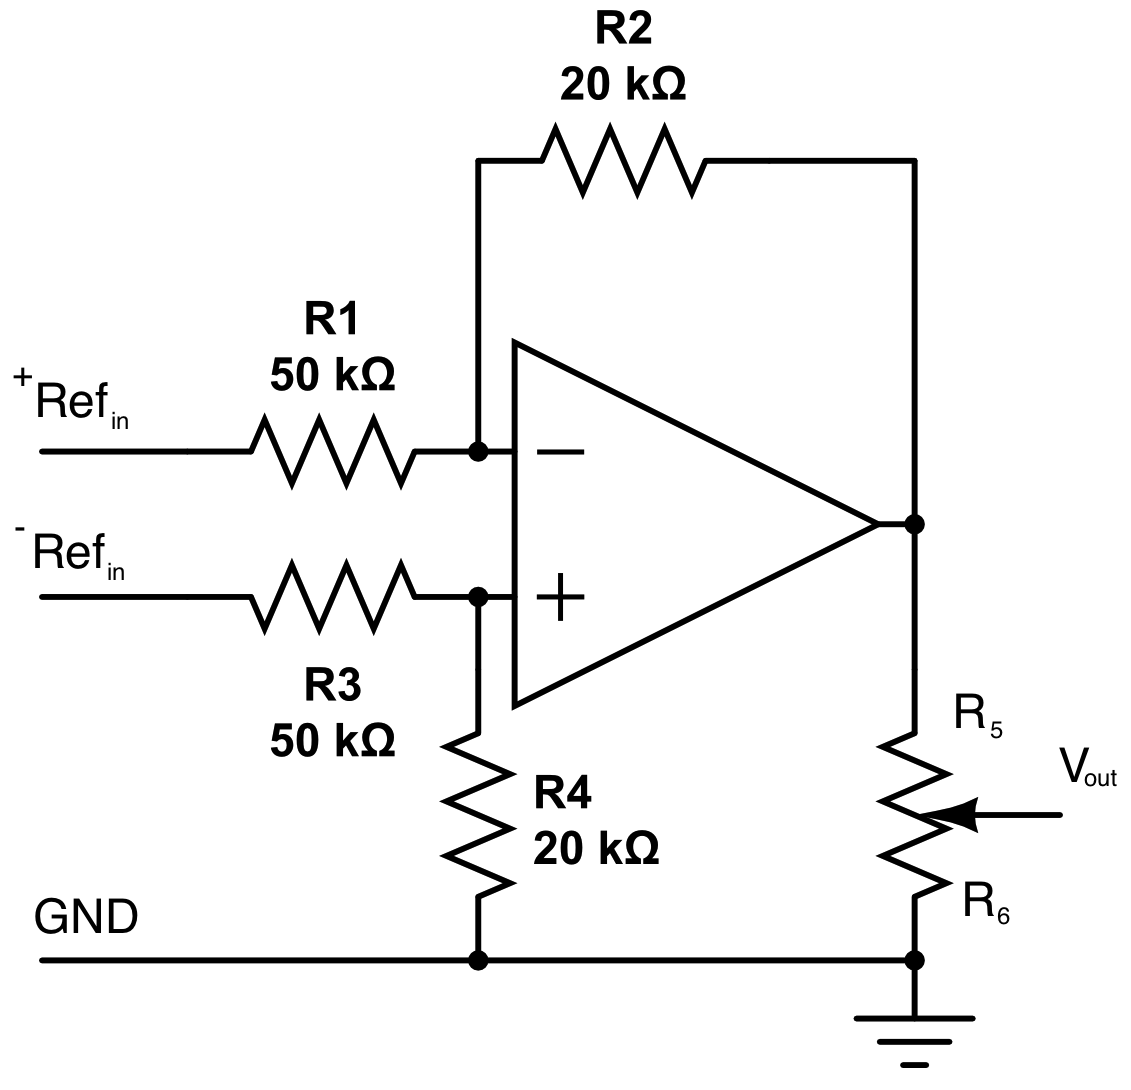
\includegraphics[width = 10cm]{q1a_u1.png}
\caption{Unit 1 within AMC servo-amplifier}
\label{q1_au1}
\end{center}
\end{figure}

\subsubsection*{U3}

U3 serves as an inverting amplifier which can be tuned by the potentiometer.

$$U3_{out} = - \left( \frac{R_3 + R_4}{R_4} \right) \left( \frac{R_2}{R_1} \right) Ref_{gain} $$
$$U3_{out} = - \left( \frac{R_3 + R_4}{R_4} \right) \left( \frac{10}{5} \right) Ref_{gain} $$

\begin{figure}[htb]
\begin{center}
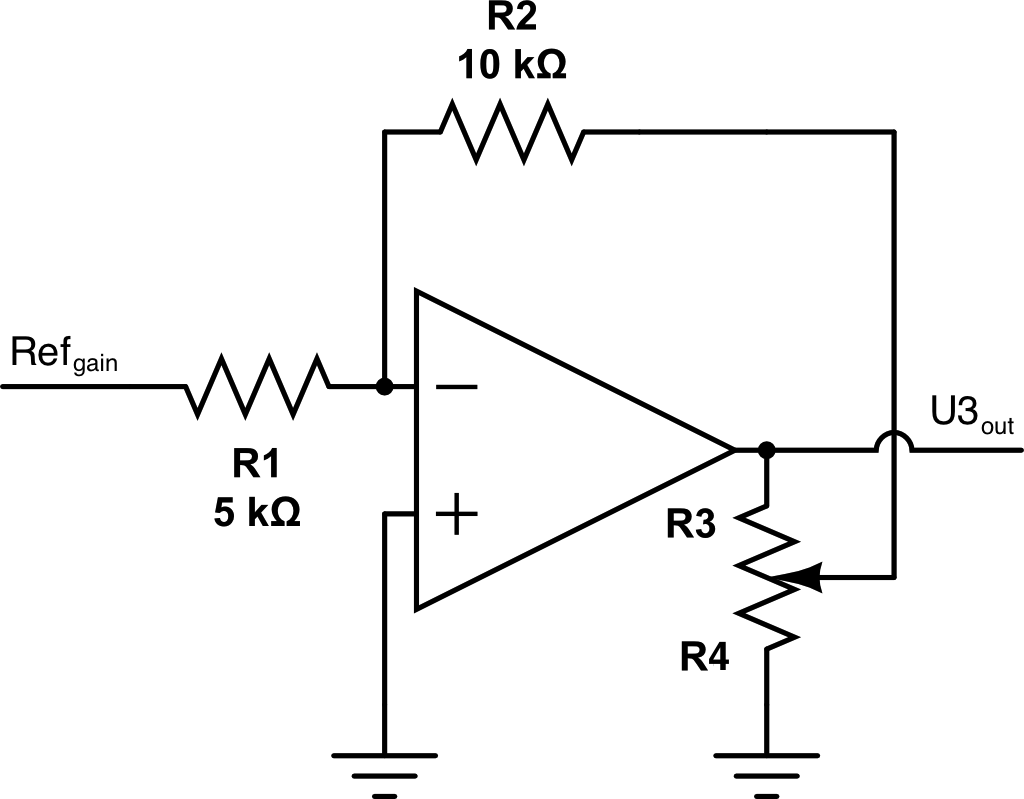
\includegraphics[width = 10cm]{q1a_u3.png}
\caption{Unit 3 within AMC servo-amplifier}
\label{q1_au3}
\end{center}
\end{figure}

\subsubsection*{U4}

U4 serves as an inverting integrator with a proportional gain when switch 3 is open, and a simple inverting amplifier with the switch closed.

$$U4_{out} = - \left( \frac{1}{R_1} \right) \left( R_2 + \frac{C_1}{s} \right) U3_{out} $$
$$U4_{out} = - \left( \frac{1}{500} \right) \left( 500 + \frac{0.01}{s} \right) U3_{out} $$

\begin{figure}[htb]
\begin{center}
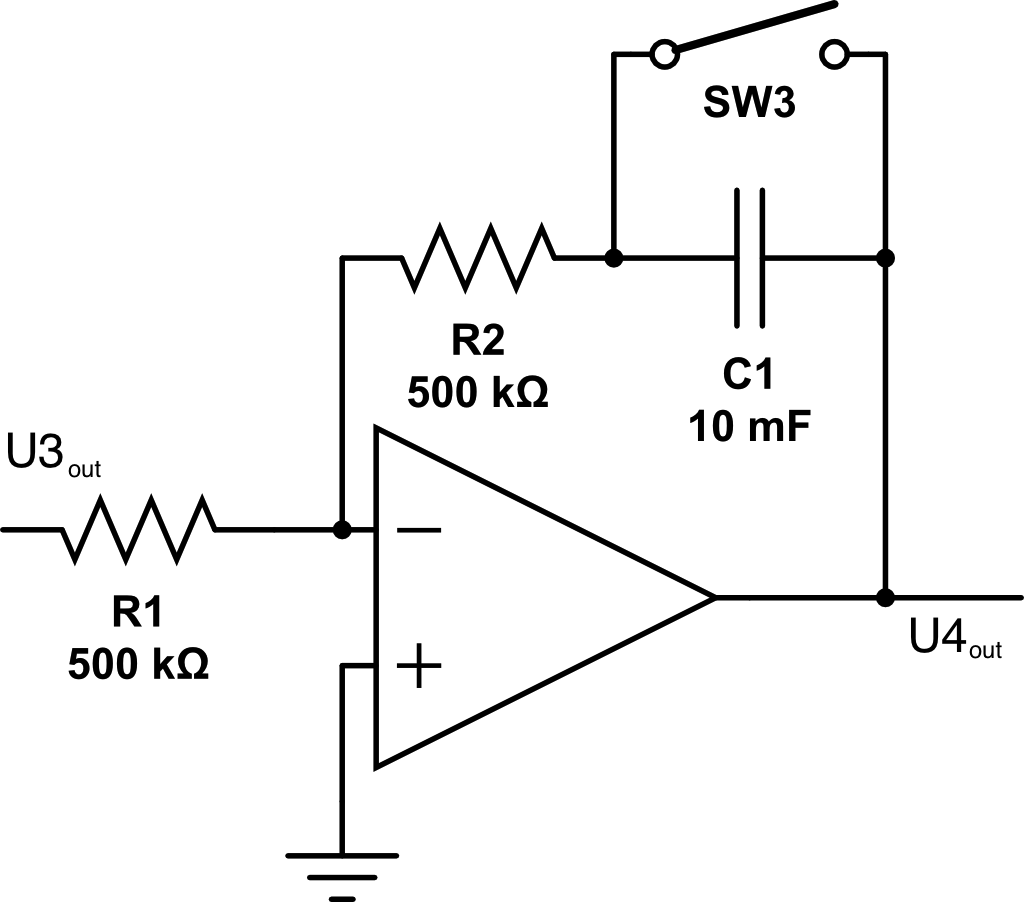
\includegraphics[width = 10cm]{q1a_u4.png}
\caption{Unit 4 within AMC servo-amplifier}
\label{q1_au4}
\end{center}
\end{figure}

\subsection*{b.}
This resistor serves to limit the current that flows through this section of the circuit to the ground because the inductor which is.  A larger resistance value decreases this current and waste less power.

\subsection*{c.}
The motor data sheet specifies a max winding temperature of $155^\circ$C, above which the motor can become irreparably damaged, and a thermal impedance of $11.2 \, \sfrac{^\circ C}{W}$.  Assuming a room temperature of $15^\circ$C, the motor's temperature can only increase by $130^\circ$C before overheating. With these values and the motor's internal resistance of $1.85 \, \Omega$, we can solve for the maximum continuous current:

$$130 = 11.2*i_{continuous}^2*1.85$$
$$i_{continuous} = 2.5048 \,A$$

With this current and the given motor constant we can then calculate the maximum continuous torque:

$$T_{m} = k_{t}*i_{continuous} = 4.24\e{-2}*2.5048 = 10.6\e{-2}\, Nm$$

This value is greater than the torque value given in the data sheet, implying that our calculated current value is less conservative than the ratings in the data sheet. Based on the given rating for max continuous torque, $8.1 \e{-2}\, Nm$, the max continuous current would be $1.91 A$, but at that value the temperature rise would be $75^\circ$C above ambient. This means that at the max torque given by the data sheet, the motor would be well under the temperature limit. It's possible that the given value is either based on a safety factor to prevent overheating, or there are other modes of breakdown that can result from higher currents. If the lower limit is based on temperature, then we should be able to use slightly higher currents given that we are running for short periods.\\

The motor's data sheet lists a peak current rating of 13.0 $A$ and a stall torque of 0.54 $N \cdot m$. With this torque value and the given torque constant (4.24$\e{-2} \sfrac{(N \cdot m)}{A}$), the peak current should be:


$$i_{peak} = \frac{T_{stall}}{k_{t}} = \frac{0.54}{4.24\e{-2}} = 12.74 \,A$$

This is less than the given rating for peak current. At this peak current limit, the motor dissipates approximately 300 W.  If the system were allowed to run at this current, and assuming that the motor does not fail in some way, it would reach a steady state temperature of:

$$P = i_{peak}^2 * R_{m} = 12.74^2 * 1.85 = 300.269 \,W$$

$$\Delta Temp = P * R_{t} = 300.269 * 11.2 = 3363.0128  \,{^\circ}C\;(above \;ambient)$$ 

Clearly the system could not physical reach this temperature without failing, but it illustrates the reason that peak current can only be sustained for short times. With the given thermal time constant of 13.8 min, we can plot the temperature rise of the motor, as shown in figure \ref{temperature}, and estimate that it would overheat after approximately 32.4 seconds at peak current. 

\begin{figure}[htb]
\begin{center}
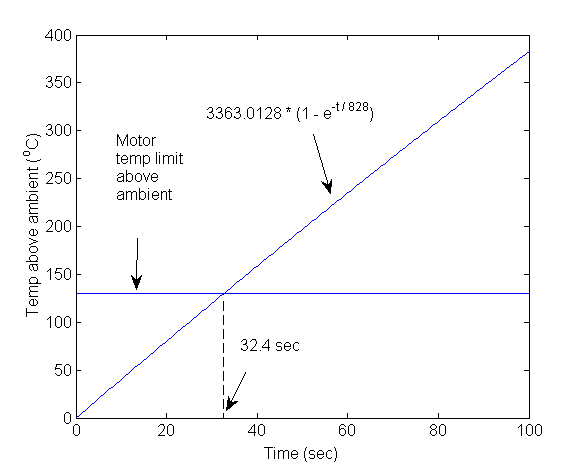
\includegraphics[width = 12cm]{temperature.png}
\caption{Motor temperature over time at peak current}
\label{temperature}
\end{center}
\end{figure}

\subsection*{d.}
The 12A8E servo amplifier is capable of outputting maximum continuous and peak currents of $\pm 6A$ and $\pm 12A$, respectively (from the data sheet). However, the servo amplifier includes a potentiometer that can be used to reduce both the continuous and peak currents while maintaining a 1:2 relationship between them. The lab instructions specify that the potentiometer should be adjusted so that the current limits will be $\pm 3A$ and $\pm 6A$.  The continuous current limit can be further reduced, without affecting the peak current, by connecting a current limiting resistor between pins P1-10 and P1-2 on the servo-amp. That was not done in this lab. Assuming the adjustment on the current limiting potentiometer was done correctly, the servo-amp should be capable of sending $\pm 3A$ continuously and $\pm6A$ intermittently to the motor. The continuous current limit from the servo-amp is greater than the continuous current rating of the motor, so we can't rely on the servo-amp to prevent the motor from drawing too much current.\\


The data sheet for the servo-amp specifies a peak current of $\pm12 A$ for a maximum of 2 seconds. From information on the Advanced Motion Controls website, this can only be achieved if the current switches across its entire range (-12 A to +12 A, and vice-versa). Any change of smaller magnitude will not be maintained as long (i.e. switching from 0 A to +12 A will only be held for 1 second before the current begins falling). The primary concern with maintaining high currents is overheating, and the servo-amp has a much lower temperature limit than the motor (65 $^\circ$C vs 155 $^\circ$C), as well as a much smaller thermal time constant than the motor.  This is why the peak current can not be maintained for long, the maximum temperature would be exceeded very quickly and the servo-amp's internal safeties would shut it off. As an example, in the thermal model for the motor at peak current (which is lower than the 6 A rating of the servo-amp), 65 $^\circ$C was reached in only 9.8 seconds. Of course, the servo-amp has different thermal properties than the motor, so that specific value is not accurate. However, the basic idea is valid: the servo-amp is capable of passing a lot of current, and has a lower temperature limit than the motor, so there is a danger of it overheating if high currents are maintained. Luckily, the servo-amp has built in safeties, such as a thermal shut-off.  \\

\subsection*{e.}
In the above sections, we showed that the motor has a continuous and peak current limits of 2.5 A and 12.74 A, and the servo-amp  has current limits of 3 A and 6 A, respectively. Within our LabView controller we chose to implement saturation limits of $\pm6$ A so that we could take advantage of the peak current capability of the servo-amp and motor. We considered setting a saturation limit based on the motor's continuous current limit of 2.5 A, but felt that might have a negative effect on the transient response of the motor. Also, we knew that the servo-amp has built in mechanisms to prevent the current from remaining at the peak value - it automatically lowers it after at most two seconds. Additionally, as we were tuning our LabView controller, we monitored a waveform graph of the attempted output of the controller. This allowed us to adjust our gain values not just for system stability, but also to keep the attempted output within safe limits. Given more resources, we could have implemented more safety measures. For example, we could implement a slow-blow fuse rated a little under the continuous current limit of the motor. This would protect the system from high currents for prolonged times, but still allow for short bursts of higher current during transient conditions.\\

\clearpage

\section*{2.}

\subsection*{a.}

Using expressions for the back-emf of the motor along with a simple electrical model of the motor as a resistance in series with an inductance we can model the motor-driver circuit.   This derivation neglects the effects of changing current direction in the rotor windings during operation. We can combine this electrical model with a simple lumped parameter model of physical dynamics of the motor to derive an overall transfer function.  
$$V_{s} - e = iR + L\left(\frac{di}{dt}\right) \hspace{1cm} e = K_{b} \dot{\theta} $$

$$ \Sigma_{\tau} = \tau_{motor} - \tau_{damping} + \tau_{coulomb} = J \ddot{\theta}$$
$$ \tau_{motor} = K_{T}i \hspace{1cm} \tau_{damping} = b \dot{\theta}$$

\[
  \tau_{coulomb} = \left\{
  \begin{array}{c l}
	 - \tau_{motor} & \quad \text{if } \dot{\theta} = 0 \text{ and } |\tau_{motor}| < \tau_{friction} \\
	- sgn(\tau_{motor}) \cdot \tau_{friction} & \quad \text{if } \dot{\theta} = 0 \text{ and } |\tau_{motor}| > \tau_{friction} \\
	- sgn(\dot{\theta}) \cdot \tau_{friction} & \quad \text{if } \dot{\theta} \neq 0 \\
%    	- \mu_{kinetic}N & \quad \text{if } \dot{\theta} > 0 \\
%    	+ \mu_{kinetic}N & \quad \text{if } \dot{\theta} < 0 \\
%	- \mu_{static}N & \quad \text{if } \dot{\theta} = 0 \text{ and } \tau_{motor} > \mu_{static}N \\
%	- \tau_{motor} & \quad \text{if } \dot{\theta} = 0 \text{ and } 0 <= \tau_{motor} <= \mu_{static}N \\
%	+ \mu_{static}N & \quad \text{if } \dot{\theta} = 0 \text{ and } \tau_{motor} < -\mu_{static}N \\
%	+ \tau_{motor} & \quad \text{if } \dot{\theta} = 0 \text{ and } 0 >=\tau_{motor} >= -\mu_{static}N \\
  \end{array} \right.
\]

Where: $K_{t}$ is the motor torque constant; $J$ is the rotor inertia; $b$ is the viscous damping on the rotor; $K_{b}$ is the back-emf constant of the motor; $R$ is the equivalent resistance of the motor; $L$ is the effective motor inductance; $i$ is the current flowing through the motor; and $\tau_{coulomb}$ is the force of coulomb friction on the rotor. \\

Neglecting coulomb friction:

$$ V_{s}(s) - s \, K_{b} \, \theta (s) = I(s) (R+sL) \hspace{1cm} \text{and} \hspace{1cm} K_{t} \, I(s) = \theta(s)(Js^2+bs) $$
$$ \frac{\theta(s)}{V(s)} = \frac{K_T}{s\left[ (Js + b)(Ls + R)+K_bK_T \right]} $$

The transfer function relating voltage and position is not particularly convenient and a much simpler one can be constructed relating motor current, $I(s)$, and angular position, $\theta (s)$. 

$$ K_{t} \, I(s) = \theta(s)(Js^2+bs) $$
$$ \frac{\theta(s)}{I(s)} = \frac{K_T}{(Js + b)s} $$

This model relating angular position with motor current requires the moment of inertia of the rotor, $J$, the viscous damping coefficient, $b$, and the torque constant $K_T$.  Note that coulomb friction has been neglected.  The driver operating in current mode gives us control over the torque exerted by the motor as long as the we avoid saturating our supply voltages of $\pm 24 V$.  This saturation occurs because without an external load on the motor, the rotor is free to spin up to a high angular velocity only limited by viscous damping and coulomb friction.  At these high velocities, the back emf across the motor increases, meaning that the driver must supply higher voltages across the motor to pass the same current through it.\\

\begin{figure}[htb]
\begin{center}
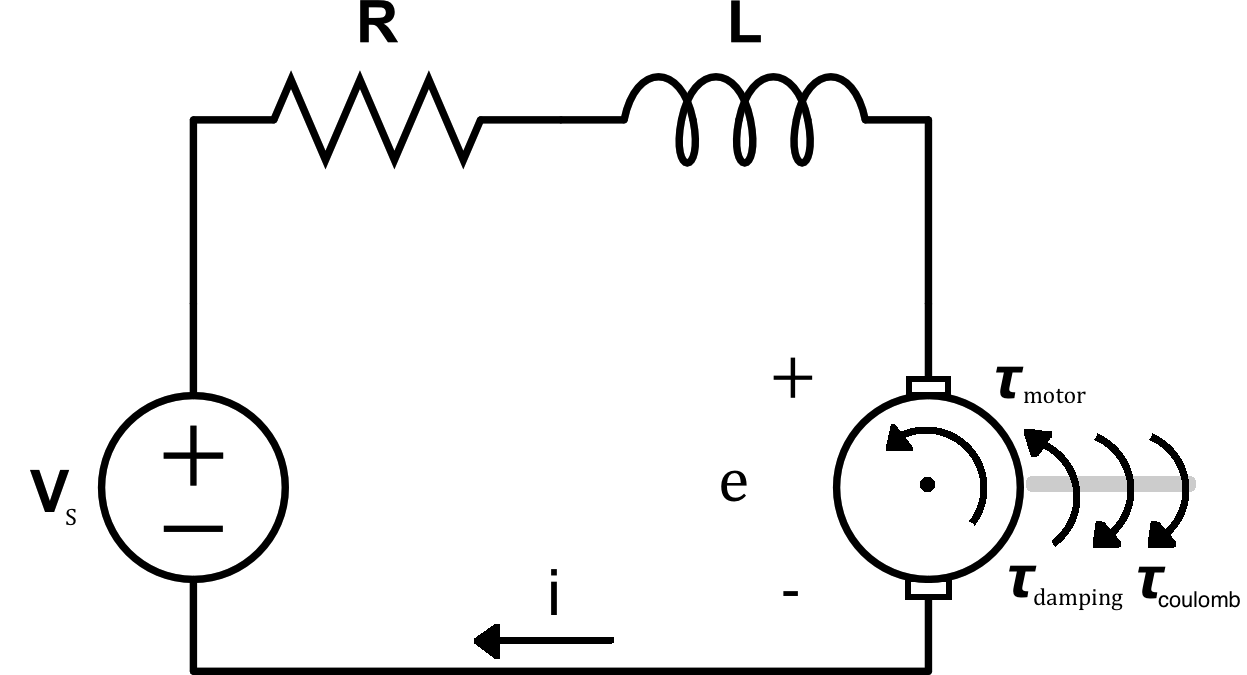
\includegraphics[width = 13cm]{dcmotor.png}
\caption{DC motor model.  Note that the sign convention here is not the one used in the remainder of the report, but is presented to concisely reflect the nature of the system.}
\label{q2_a1}
\end{center}
\end{figure}

\subsection*{b.}

The torque of friction and the viscous damping can be jointly  derived in an experiment where for a given constant input voltage to the driver, $V_{driver}$, we read off the steady state angular velocity, $\dot{\theta}_{ss}$.  At a constant velocity the following equation holds giving a relationship between $\tau_{motor}$, $b$, and $\tau_{coulomb}$.

$$\Sigma_{\tau} =  \tau_{motor} - b\dot{\theta} + \tau_{coulomb} = J \ddot{\theta} \hspace{1cm} \ddot{\theta} = 0 $$
$$ \tau_{motor} = K_{T}I_{m} = b\dot{\theta}_{ss} - \tau_{coulomb}$$

Assuming that we have the motor torque constant $K_{t}$, we can write a linear equation that relates steady state angular velocity $\theta_{steady state}$ to motor current which is assumed to be directly proportional to $V_{driver}$ for suitably small values of $V_{driver}$.

$$ V_{driver} = I_{m} \hspace{1cm} V_{driver} = \left( \frac{b}{K_T} \right) \dot{\theta}_{ss} - \frac{\tau_{coulomb}}{K_{T}} $$

From our plot in figure \ref{q2_b4} we can obtain $\left( \sfrac{b}{K_t} \right)$ as the slope of each of the linear segments and $\sfrac{\tau_{coulomb}}{K_{T}}$ as the y intercepts shown in table \ref{q2_b5}.  We can separately determine the force of static friction $\tau_{static \, coulomb}$ by measuring the smallest input voltage to the driver, and from this how much torque, is required to start the motor from rest.

$$ \Sigma_{\tau} =  \tau_{motor} - b\dot{\theta} + \tau_{coulomb} = J \ddot{\theta} \hspace{1cm} \dot{\theta} = \ddot{\theta} = 0 $$
$$ V_{driver} = - \frac{\tau_{coulomb}}{K_{T}} $$

\begin{figure}[htb]
\begin{center}
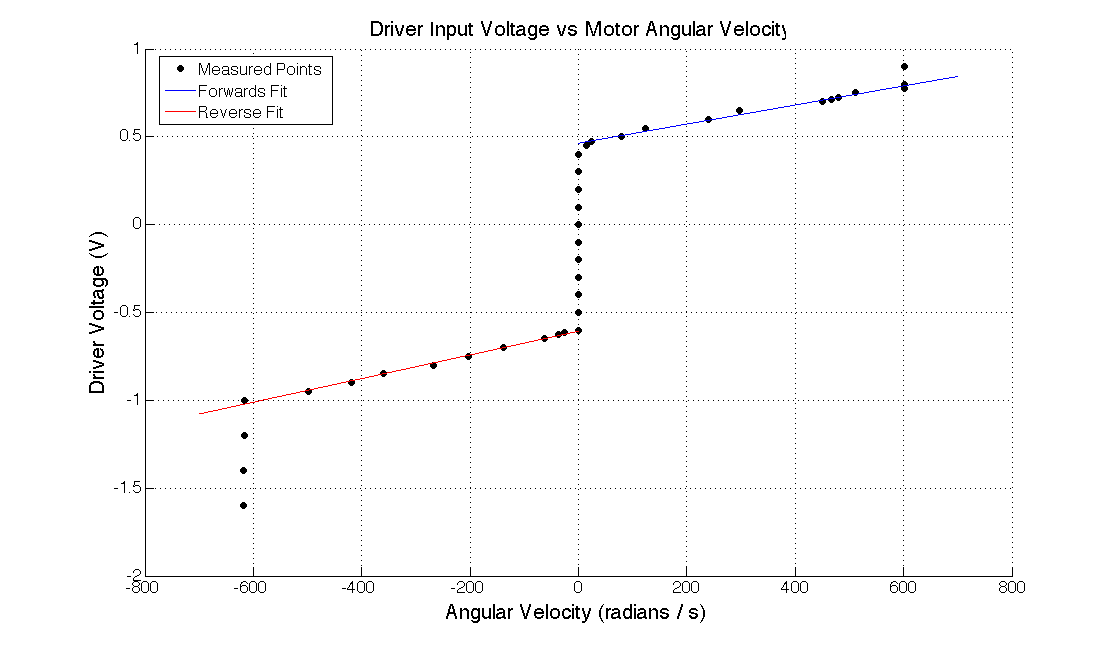
\includegraphics[width = 16cm]{SpeedCurrentCurve.png}
\caption{Relationship between angular velocity and steady state voltage applied to motor driver.  Notice the saturation at $\pm 600 \, \sfrac{radians}{s}$}
\label{q2_b4}
\end{center}
\end{figure}

\begin{table}[htb]
\begin{center}
    \begin{tabular}{|c|c|c|}
        \hline
        ~        & Slope $\left( \frac{V * s}{rad} \right) $ & y-intercept $ \left( V \right) $ \\ \hline
        Forwards & 5.4289e-04                                & 0.46374                          \\ 
        Reverse  & 6.72805e-04                               & -0.60717                         \\
        \hline
    \end{tabular}
\end{center}
\caption{Extracted slopes and y-intercepts from current speed curve}
\label{q2_b5}
\end{table}

If we assume the motor constant on the data-sheet of $0.0424 \, \sfrac{(N \cdot m)}{A}$ then we can arrive at the following estimates for b and $\tau_{coulomb}$, shown in table \ref{q2_b10} compared against the values obtained from the data sheet.  Our values are within an order of magnitude of the provided values which is not close enough to make any particular claims besides that this motor seems to have worse performance than advertised. \\

\begin{table}
\begin{center}
    \begin{tabular}{|c|c|c|}
        \hline
        ~                                                        & Data Sheet Values   & Average Estimated Values \\ \hline
        $b \, \left( N \cdot s \right) $             & $3.7 \cdot 10^{-6}$ & $2.5773 \cdot 10^{-5}$   \\ 
        $\tau_{coulomb} \, \left( N \cdot m \right)$ & $5.6 \cdot 10^{-3}$ & $0.044978$               \\
        \hline
    \end{tabular}
\end{center}
\caption{Comparison of viscous damping and friction torque estimates with values obtained from the data sheet}
\label{q2_b10}
\end{table}

To compute the torque constant, $K_{T}$ we can first compute the back-emf constant, $K_b$, which we know to be numerically equal to $K_T$ in SI units.  To calculate $K_b$ we can measure the internal resistance of the motor, R, using an ohm-meter.  Then running the system at a constant current, we can measure the source voltage, $V_{s}$ that the driver outputs to maintain that current to obtain e. We can use the encoder to measure the angular velocity and use that value with e to solve for $K_b$:

$$ \Sigma_{V} = V_{s} + V_{R} + V_{L} e = V_{s} + IR + e = 0 $$
$$ K_b = \frac{e}{\dot{\theta}} $$

%To determine the torque constant, we can place the motor on its side, pin a pulley to the shaft and attach a known mass to the pulley.  This exerts a known torque on the shaft, and we can simply adjust motor current until it balances out the torque.   
%
%$$ \Sigma_{tau} = \tau_{motor} - b\dot{\theta} + \tau_{coulomb} - \tau_{mass}= J \ddot{\theta} \hspace{1cm} \dot{\theta} = \ddot{\theta} = 0  $$
%$$ \tau_{motor} = - \tau_{coulomb} + \tau_{mass} \approx \tau_{mass} $$
%
%$$ K_T \approx \frac{\tau_{mass}}{i_{equilibrium}} = \frac{mg(r_{pulley})}{i_{equilibrium}} $$

%We can experimentally determine the viscous damping term, $b$ by applying a known torque to the motor.  Once the angular velocity has reached steady state, $b$ can be read off directly.  The driver in current mode delivers a known current, which using the torque constant determined above yields the torque.  
%
%$$ \Sigma_{tau} = \tau_{motor} - b\dot{\theta} + \tau_{coulomb} = J \ddot{\theta} \hspace{1cm} \ddot{\theta} = 0 $$
%$$ b = \frac{\tau_{motor} + \tau_{coulomb}}{\dot{\theta}} \approx \frac{\tau_{motor}}{\dot{\theta}}$$

We can determine the moment of inertia of the rotor, $J$ by starting from rest and sending the motor a known torque while recording the position as a function of time stopping when the system has reached a constant velocity.  Then by computing the $1^{st}$ and $2^{nd}$ order derivatives at each time step we can assemble a linear system to allow us to jointly solve for $J$, $b$, and $\tau_{coulomb}$.

$$ A_{t} = \left[ \begin{array}{c c c} \ddot{\theta_{t}} & \dot{\theta_{t}} & -1 \end{array} \right]  \hspace{1cm} 
x = \left[ \begin{array}{c} J \\ b \\ \tau_{coulomb} \end{array} \right] \hspace{1cm} z_{t} = \tau_{motor} $$
$$ Ax = z $$

Rather than attempt the method above, we instead used MATLAB's numerical differential equation solving to simulate the trajectory of the system as a function of time, driver current, $I_t$ and our unknown system parameters $J$, $b$, $K_t$, and $\tau_{coulomb}$.  By then
comparing the predicted angular positions with the measured angular positions over time, we can construct a non-linear regression to estimate the unknown parameters.  We collected a data set where the driver was given a sinusoidal voltage, and we assume that motor current, $I_m$, is identical to this driver voltage and recorded the motor motion that this input caused. \\

Table \ref{q2_b1} below shows the parameters for our equation of motion obtained from the data sheet.  The results, in figure \ref{q2_b2} shows the estimated trajectory using these parameter values.  It is clear that these parameter values are quite far off.  Attempting to perform nonlinear optimization on our model parameters proved to be difficult, so we resorted to parameter sweeping to to identify appropriate starting points for regression.  Figure \ref{q2_b7} shows one of the best results discovered by this parameter sweep.  In this case the error has been reduced, but the fit still appear inappropriate.  \\

\begin{table}[htb]
\begin{center}
    \begin{tabular}{|c|c|}
        \hline
        ~                                                      & Data Sheet Parameters        \\ \hline
        $J \hspace{0.1cm} \left( \frac{N\cdot s^2}{m} \right)$     & $8.5 \cdot 10^{-6} $               \\ 
        $b \hspace{0.1cm} \left( N \cdot s \right) $               & $3.7\cdot 10^{-6} $                 \\ 
        $\tau_{coulomb} \hspace{0.1cm} \left( N \cdot m \right)$           & $5.6 \cdot 10^{-3}$  \\ 
        $K_{T} \hspace{0.1cm} \left( \frac{N\cdot m}{A} \right) $ & $4.24 \cdot 10^{-2}$             \\
        \hline
    \end{tabular}
\caption{Original model parameter values obtained from the data sheet.}
\label{q2_b1}
\end{center}
\end{table}

\begin{figure}[htb]
\begin{center}
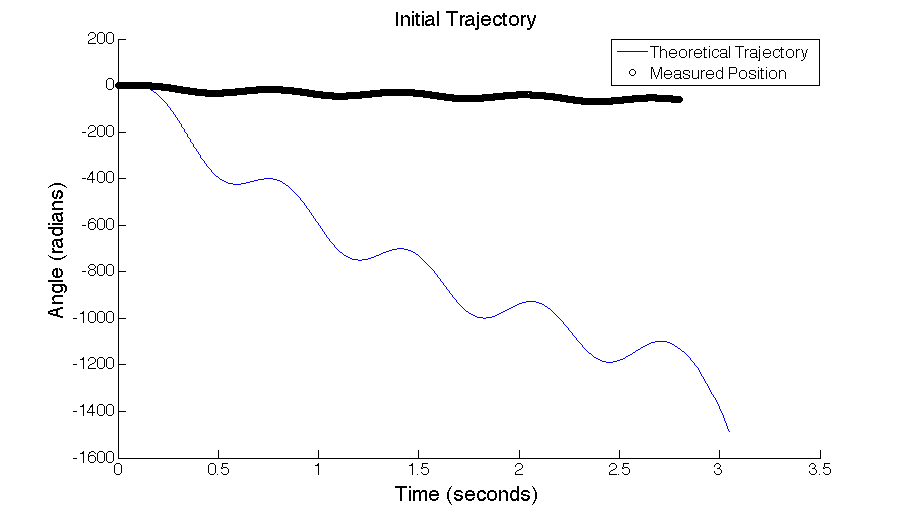
\includegraphics[width = 14cm]{initialModel.png}
\caption{Predicted behavior vs Actual behavior using initial parameter values noted in table \ref{q2_b1}.}
\label{q2_b2}
\end{center}
\end{figure}

\begin{figure}[htb]
\begin{center}
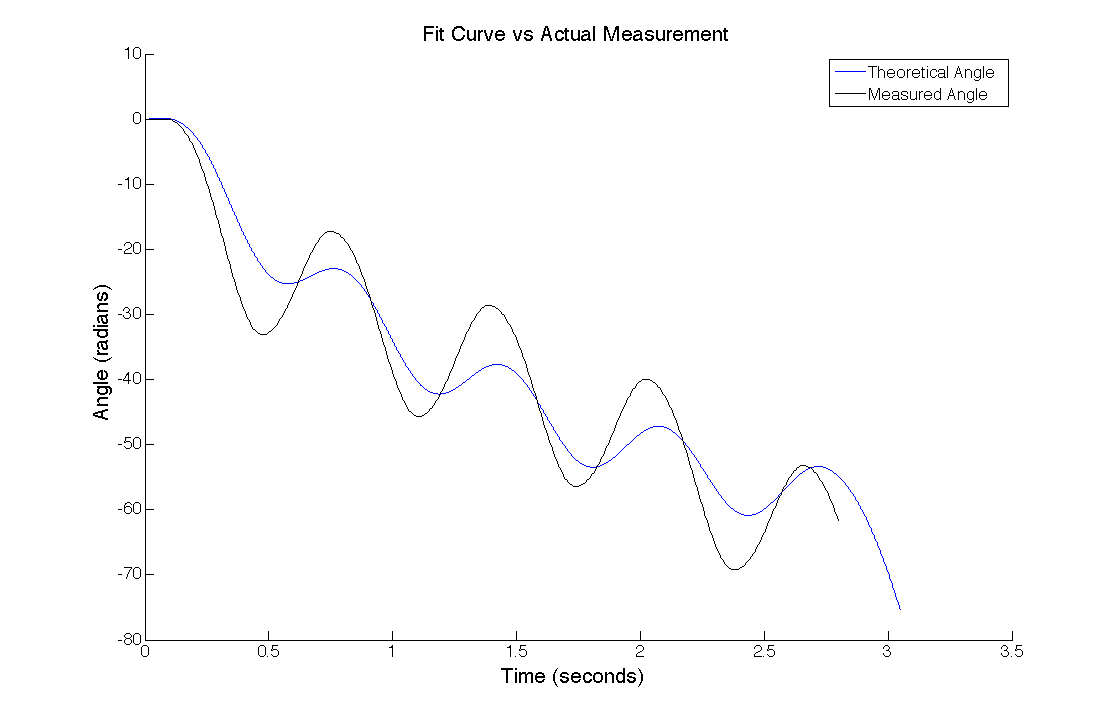
\includegraphics[width = 14cm]{2ndexamplefit.png}
\caption{Fit by non-linear optimization and parameter sweeping: $J = 6.06724 \cdot 10^{-5} \, B = 4.05562 \cdot 10^{-5} \, F_{f} = 1.45312 \cdot 10^{-4} \, K_{t} = 0.019020 $}
\label{q2_b7}
\end{center}
\end{figure}

Manual parameter guessing revealed that it was not possible to obtain the measured curve using the model, repeated below. 
$$ \Sigma_{tau} = K_{T}I_{m} - b\dot{\theta} + \tau_{coulomb} = J \ddot{\theta} $$

Clearly there were some effects that this model neglected.  Our previous experiment to attempt to determine $b$ and $\tau_{coulomb}$ showed that these parameters are likely not the same in each direction, so we augmented the model to allow $b$ and $\tau_{coulomb}$ to take on different values in the forwards direction and reverse directions yielding the following model:

$$ \Sigma_{tau} = \tau_{motor} - b\dot{\theta} + \tau_{coulomb} = J \ddot{\theta} $$

\[
  \tau_{coulomb} = \left\{
  \begin{array}{l l}
    	- \tau_{forwards} & \quad \text{if } \dot{\theta} > 0 \\
    	+ \tau_{reverse} & \quad \text{if } \dot{\theta} < 0 \\
	- \tau_{forwards} & \quad \text{if } \dot{\theta} = 0 \text{ and } \tau_{motor} > \tau_{forwards} \\
	- \tau_{motor} & \quad \text{if } \dot{\theta} = 0 \text{ and } 0 <= \tau_{motor} <= \tau_{forwards} \\
	+ \tau_{reverse} & \quad \text{if } \dot{\theta} = 0 \text{ and } \tau_{motor} < -\tau_{reverse} \\
	+ \tau_{motor} & \quad \text{if } \dot{\theta} = 0 \text{ and } 0 >=\tau_{motor} >= -\tau_{reverse}\\
  \end{array} \right.
\]

\[
b = \left\{
\begin{array}{l l}
b_{forwards} & \quad \text{if } \dot{\theta} > 0 \\
b_{reverse} & \quad  \text{if } \dot{\theta} < 0 \\
\end{array} \right.
\]

With this improved model and some intelligent guessing for new parameter values, we arrived at an excellent fit shown in figure \ref{q2_b3}. The most notable feature of these values is the large difference between the torque of friction in the forwards and reverse directions. \\ 

\begin{table}[htb]
\begin{center}
    \begin{tabular}{|c|c|c|}
        \hline
        ~                 & Data-Sheet Values    & Fit Values              \\ \hline
        $J \hspace{0.1cm} \left( \frac{N \cdot s^2}{m} \right)$               & $8.5 \cdot 10^{-6} $     & $3.50514 \cdot 10^{-5}$ \\ 
        $K_{t} \hspace{0.1cm} \left( \frac{N\cdot m}{A} \right)$           & $0.0424$             & $0.0314499$             \\ 
        $b_{forwards} \hspace{0.1cm} \left( N \cdot s \right)$    & $3.7 \cdot 10^{-6} $ & $1.08586 \cdot 10^{-5}$ \\ 
        $b_{reverse} \hspace{0.1cm} \left( N \cdot s \right)$     & $3.7 \cdot 10^{-6} $ & $4.85930 \cdot 10^{-5}$ \\ 
        $\tau_{forwards} \hspace{0.1cm} \left( N \cdot m \right)$ & $5.6 \cdot 10^{-3}$  & $0.0224389$             \\ 
        $\tau_{reverse} \hspace{0.1cm} \left( N \cdot m \right)$   & $5.6 \cdot 10^{-3}$  & $0.0143096$             \\
        \hline
    \end{tabular}
\caption{Final Parameter Values vs Original Data Sheet Values}
\label{q2_b8}
\end{center}
\end{table}

Table \ref{q2_b8} shows our final fit values alongside the original values obtained from the data sheet, while the fit curve itself is shown in figure \ref{q2_b3}.  This large difference in values is clearly illustrated by the large difference in behavior between the actual system and our model using the values obtained from the data sheet shown in figure \ref{q2_b2}.  \\

We can also compare these fit values with values obtained from our earlier experiment, shown together in table \ref{q2_b9}, after adjusting for the difference in motor torque constant, and notice that our terms are quite similar, however it seems as if this experiment did not accurately estimate the force of friction as the relative values seem to be flipped between the two experiments.\\

\begin{table}[htb]
\begin{center}
    \begin{tabular}{|c|c|c|}
        \hline
        ~                 & Predicted Value          & Fit Value               \\ \hline
        $B_{forwards}$    & $1.707338 \cdot 10^{-5}$ & $1.08586 \cdot 10^{-5}$ \\ 
        $B_{reverse}$     & $2.11611 \cdot 10^{-5}$  & $2.49301 \cdot 10^{-5}$ \\ 
        $\tau_{forwards}$ & $0.0145846$              & $0.0224389$             \\ 
        $\tau_{reverse}$  & $0.0190954$              & $0.0143096$             \\
        \hline
    \end{tabular}
\caption{Damping and friction torques calculated from earlier experiment vs fit values}
\label{q2_b9}
\end{center}
\end{table}

\begin{figure}[htb]
\begin{center}
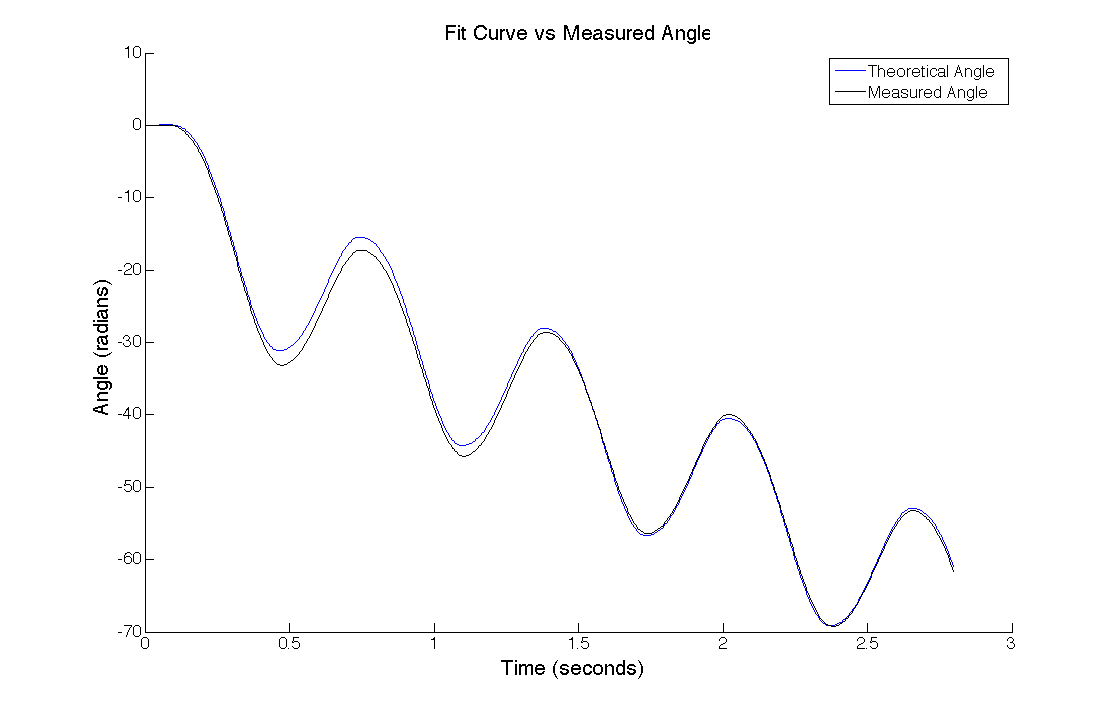
\includegraphics[width = 14cm]{awesomefitFiner.png}
\caption{Predicted behavior vs Actual behavior using fit parameter values and enhanced modeling}
\label{q2_b3}
\end{center}
\end{figure}

\clearpage

\section*{3.}
\subsection*{Simulink Model}
Figure \ref{q3_1} shows the overall model of DC motor servo system for both velocity and position control. It consists of four main units: 
\begin{itemize}
\item DC Motor
\item Optical Encoder 
\item Servo Amplifier 
\item Controller
\end{itemize}

\begin{figure}[htb]
\begin{center}
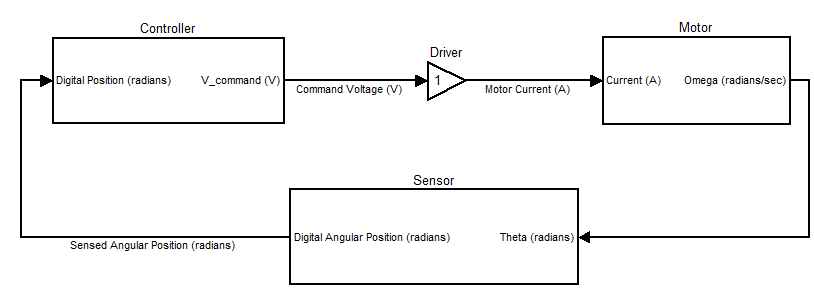
\includegraphics[width = 14cm]{q3_1}
\caption{DC motor servo system}
\label{q3_1}
\end{center}
\end{figure}

\clearpage

\subsubsection*{DC Motor}
The DC motor subsystem, seen in figure \ref{q3_2} worked on the principle that the input torque generated was based on the conversion equation: 
$$T = K_t*i$$
Where, $K_t = 4.24\times10^{-2}$  is the torque constant of the motor. According to the motor datasheet, the rotor inertia, $J$, is $8.5 \times 10^{-6}$ , and the viscous damping coefficient, $B, =3.7\times10^{-6}$.\\

Friction torque was modeled as a simple coulomb viscous model, shown in figure \ref{q3_3}. As the viscous friction was already taken into account in the motor transfer function, the model of coulomb friction was created using the following simple function: 
$$T_f^{+/-} (\omega) =T_{cou}l^{+/-}$$
Where,  Coulomb Friction Torque: $ T_f = 5.6\times 10^{-3} \ \  [Nm/A]$


\begin{figure}[htb]
\begin{center}
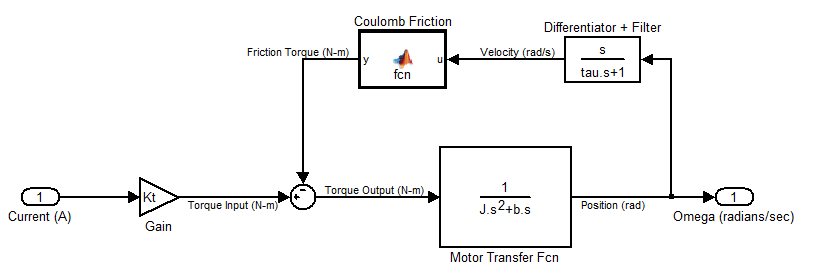
\includegraphics[width = 14cm]{q3_2}
\caption{DC Motor Subsystem}
\label{q3_2}
\end{center}
\end{figure}

\begin{figure}[htb]
\begin{center}
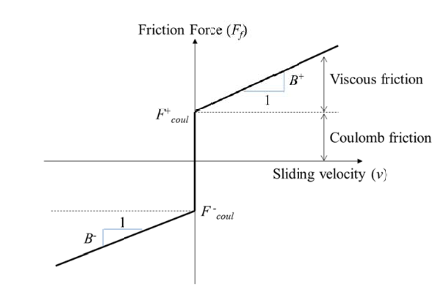
\includegraphics[width = 10cm]{q3_3}
\caption{Plot of Friction Force v.s. Velocity}
\label{q3_3}
\end{center}
\end{figure}

\clearpage

\subsubsection*{Optical Encoder}
The optical encoder (see figure \ref{q3_3}) was modeled as a quantizer with the interval size equal to $2\pi/2000$ was used to simulate the effects of the ADC.

\begin{figure}[htb]
\begin{center}
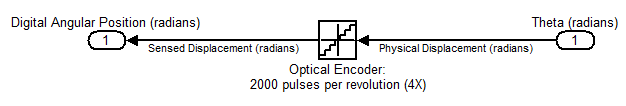
\includegraphics[width = 14cm]{q3_4}
\caption{The Optical Encoder Subsystem}
\label{q3_4}
\end{center}
\end{figure}


\subsubsection*{Servo Amplifier}
The Servo Amplifier was treated as a gain equal to 1 due to its high bandwidth (2.5 kHz). It can be seen in figure \ref{q3_1}.

\subsubsection*{Controller}
Two controllers were used to achieve both position and velocity control, they are visible in figures \ref{q3_5} and \ref{q3_6}. The saturation limit was set to $\pm 6 A$ based on the maximum peak current of the servo-amplifier. An additional concern was that the $RMS$ command voltage needed to be lower than the maximum continuous current of the motor ($1.92 A$). We ensured that limiting our output to $\pm 6$ Volts generally allowed for better tracking stability while not often applying more than $1.92 A$ for continuous periods of time.\\

Additionally PID block represents the controller while $\tau$ (tau) represents the filter time-constant for the transfer function from angular position to velocity. It was treated as a variable coefficient.\\

\begin{table}[htb]
\begin{center}
    \begin{tabular}{|c|c|c|c|c|}
        \hline
        $J$                   & $B$                   &$K_t$                   & $T_f$                  & $K_{amp}$           \\
        Rotor inertia       & Viscous damping     & Torque constant      & Friction torque     & Gain of driver \\ 
        $[kgm^2]$           & $[Nms]$             & $[Nm/A]$             & $[Nm]$              & $[A/V]$        \\ \hline
        $8.5\times 10^{-6}$ & $3.7\times 10^{-6}$ & $4.24\times 10^{-2}$ & $5.6\times 10^{-3}$ & $1$            \\
        \hline
    \end{tabular}
\end{center}
\end{table}

\begin{figure}[htb]
\begin{center}
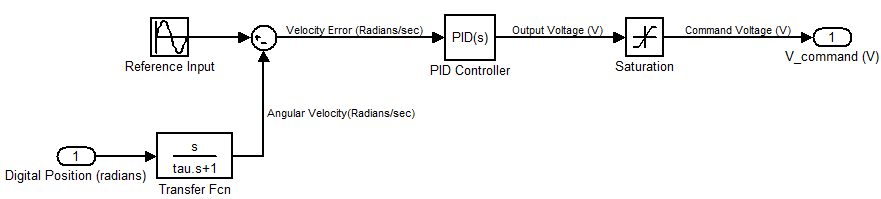
\includegraphics[height = 6 cm, width = 18 cm]{q3_5}
\caption{The Velocity Control Subsystem}
\label{q3_5}
\end{center}
\end{figure}

\begin{figure}[htb]
\begin{center}
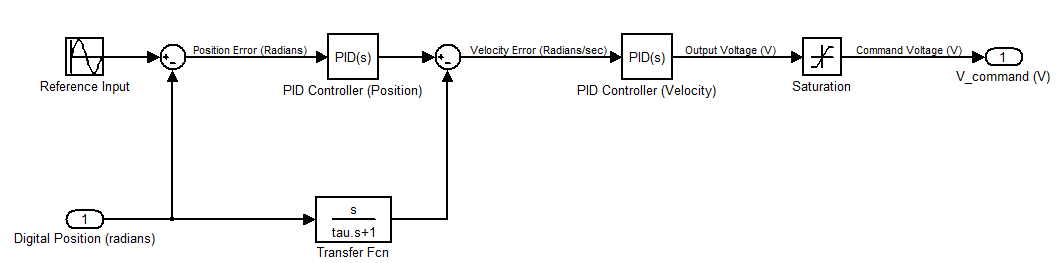
\includegraphics[height = 6 cm,width = 18 cm]{q3_6}
\caption{The Position Control Subsystem}
\label{q3_6}
\end{center}
\end{figure}

\clearpage

\subsection*{Controller Design}
The cascaded P/PI controller (see figure \ref{q3_7}) is one of the most commonly used controller structures in motion control systems. It is simple and has a systematic tuning procedure. This configuration allowed us to reuse the velocity controller within our position controller.\\

\begin{figure}[htb]
\begin{center}
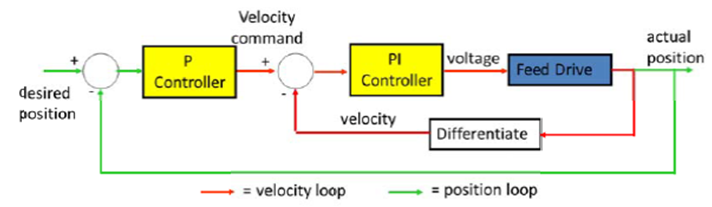
\includegraphics[width = 14 cm]{q3_7}
\caption{Basic Structure of P/PI Controller}
\label{q3_7}
\end{center}
\end{figure}

This design consists of two cascaded loops. The inner one is the velocity loop. It is a PI controller which aims to ensure that the velocity command is tracked accurately. It is surrounded by the outer position loop which is a P controller that ensures the desired reference point is achieved. Having both loops makes it easy to deal with each loop at one time. The first step is to optimize the PI controller, achieving the best performance in the velocity loop, and then tune the P controller to ensure position tracking performance.\\

\subsubsection*{Velocity Control System - Dynamics Analysis}
Before we began tuning, we needed to know the overall system dynamics, which provide essential information to guide the tuning process. Frequency response was used to analyze the velocity loop based on different values of time constant, $\tau$. The following figures (\ref{q3_8}, \ref{q3_9} and \ref{q3_10}) show Bode diagrams for the transfer functions of open-loop ($G_{OL}$), close-loop ($G_{CL}$), input disturbance rejection ($G_{di}$), and output disturbance rejection ($G_{do}$) with $\tau = 0.05, 0.1, \text{and } 1$, respectively.

\begin{itemize}
\item $G_{OL}$ (see figure \ref{q3_8}): when $\tau$ increases, the gain of $G_{OL}$ becomes lower in medium and high frequencies, so does the phase behavior. It can be observed that a larger $\tau$ may make the system unstable in lower frequencies since the phase is close to -180 degrees (smaller Phase Margin) and there are still other delays neglected by assumptions, such as the dynamics of servo amplifier.   

\item $G_{CL}$ (see figure \ref{q3_9}): the bandwidth of $G_{CL}$ decreases as $\tau$ increases. 

\item $G_{di}$ (see figure \ref{q3_9}): the bandwidth of $G_{di}$ is the same as that of $G_{CL}$ because the system is uncontrolled.

\item $G_{do}$ (see figure \ref{q3_10}): its quality in higher frequencies becomes better when $\tau$ increases.

\end{itemize}

We find that as $\tau$ increases, the quality of output disturbance rejection becomes better but this comes at the expense of and undesirable reduction in bandwidth.  In terms of our goals, high bandwidth (up to 5Hz), and good quality of disturbance rejection (60Hz noise signal) need to be achieved at the same time; therefore, the value of $\tau$ has to be carefully determined with controllers.

\begin{figure}[htb]
\begin{center}
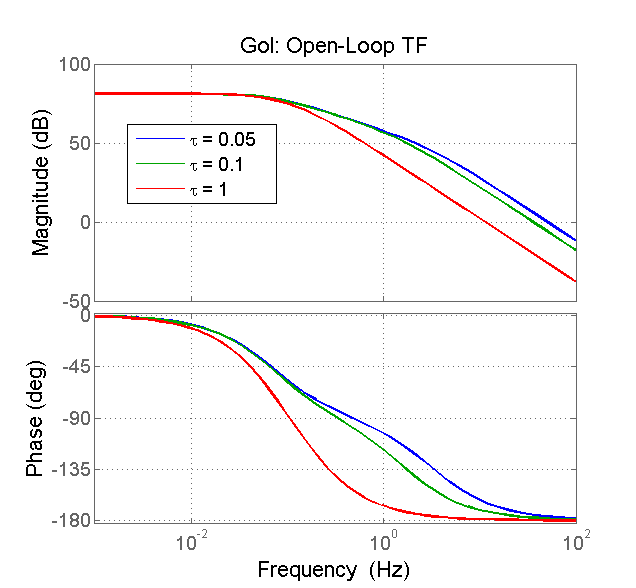
\includegraphics[width = 10 cm]{q3_8}
\caption{Changes in $G_{OL}$ as $\tau$ is increased from 0.05 to 1}
\label{q3_8}
\end{center}
\end{figure}

\begin{figure}[htb]
\begin{center}
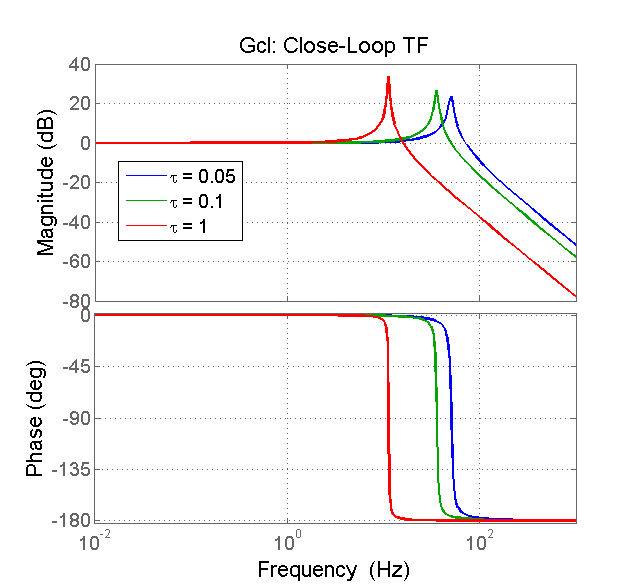
\includegraphics[width = 10 cm]{q3_9}
\caption{Changes in $G_{CL}$  and $G_{di}$ as $\tau$ is increased from 0.05 to 1}
\label{q3_9}
\end{center}
\end{figure}

\begin{figure}[htb]
\begin{center}
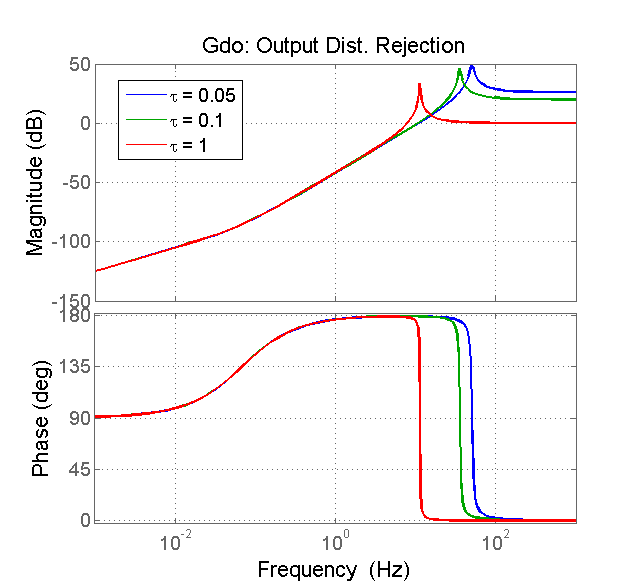
\includegraphics[width = 10 cm]{q3_10}
\caption{Changes in $G_{do}$  as $\tau$ is increased from 0.05 to 1}
\label{q3_10}
\end{center}
\end{figure}

\clearpage

\subsection*{Velocity Control System – Controller Tuning}
$$K_{VP} : \text{Proportional Gain}$$
$$K_{VI} : \text{Integral Gain}$$
$$K_{VD} : \text{Derivative Gain}$$

\subsubsection*{d) Keep steady state error below 2\% for a step command of 2$\pi$ radians/sec}
Tuning practices to achieve satisfactory step response:
\begin{itemize}
\item Initialize $\tau$ as 0.05 to begin with.
\item Tune $K_{VP}$ as high as possible because when $K_{VP}$ is increased, the crossover frequency as well as the bandwidth of velocity loop will also increase.
\item If $K_{VP}$ exceeds a certain value, it may affect the system stability or saturate either the actuator or the current driver. Considering this issue, $K_{VP}$ was limited by the maximum peak current (6A) and continuous current (1.92A), respectively. Thus, $K_{VP}$  was tuned to 15, ensuring the commanded voltage less than 1.92 A in steady state.  
\item $K_{VI}$ was not required here since the steady-state error was already less than 2\%. The reason may be because the filter seemed to provide the similar function to the integral gain.
\end{itemize}

\subsubsection*{e) Provide command tracking: Amplitude should remain within 5\% of command up until 5Hz for “command amplitude” of $\pi$/2 radians/sec}
\begin{itemize}
\item 	The tracking error of 5Hz command was up to 10\%, so that we tried to change $\tau$ to achieve better performance.
\item When $\tau$ was 0.7, the error was minimum and fluctuated below 2\%. This modification also generated better track-ability for the step input.
\end{itemize}

\subsubsection*{f) Attenuate a 60Hz noise signal coming in either at the servo-amplifier or the sensor by at least 5 times.}
\begin{itemize}
\item A noise signal with amplitude 0.1 was used to test disturbance rejection. Over 90\% of the input disturbance from the servo amplifier was rejected; while none of the output disturbance, from the sensor was rejected but, even enlarged. Thus increasing τ was required to get better results. 
\item When $\tau$ was changed from 0.7 to 6, the goal of five-times attenuation was achieved. However, we were unable to maintain sinusoidal command tracking due to the lower bandwidth. This was a trade-off which was expected.
\item Considering the limitation of the PI controller, the derivative controller was introduced to add phase lead in our control loop, broadening the bandwidth. By trial and error, finally the three objectives were achieved with the following values of the coefficients:
$$K_{VP} = 25$$
$$K_{VI} = 0$$
$$K_{VD} = 0.2  \ \ (N \footnote{Causality filter for the differentiator}=100), \text{and}$$
$$ \tau=6.6 $$

\end{itemize}

\clearpage

\subsection*{Velocity Control System – Simulation Results}

\begin{figure}[htb]
\begin{center}
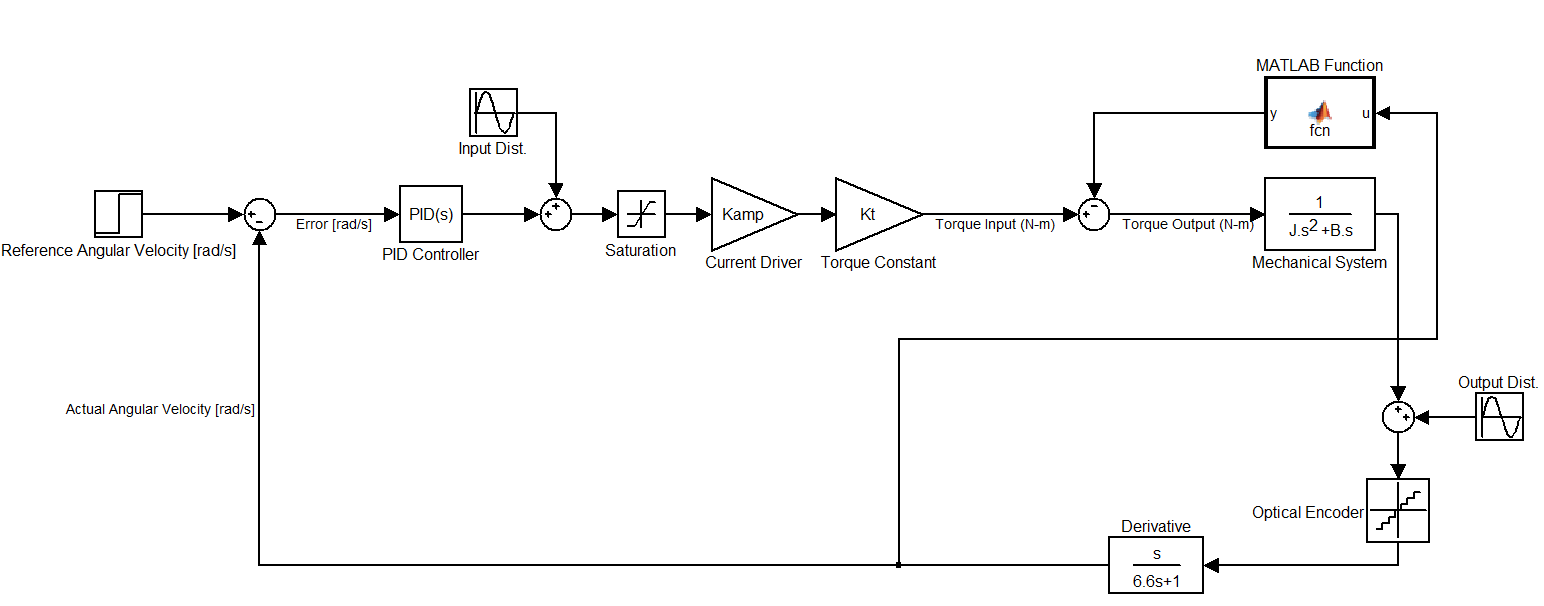
\includegraphics[height = 8 cm, width = 18 cm]{q3_11}
\caption{Block Diagram of Velocity Control system}
\label{q3_11}
\end{center}
\end{figure}

\begin{table}[htb]
\begin{center}
    \begin{tabular}{|c|c|c|c|c|}
        \hline
        $K_{VP}$ & $K_{VI}$ & $K_{VD}$ & $N$ & $\tau$ \\ \hline
        25       & 0        & 0.2      & 100 & 6.6    \\
        \hline
    \end{tabular}
\end{center}
\end{table}

\begin{table}[htb]
\begin{center}
    \begin{tabular}{|c|c|c|c|c|}
        \hline
        Reference            & Input Amplitude & Output Amplitude & \%Error & Commanded Voltage \\ 
        ~                    & [rad/s]                 & [rad/s]                  & ~       & [Max. V]                   \\ \hline
        (d)Step              & $2\pi$                  & 6.278                    & 0.08\%  & 0.15                       \\ 
        (e)Sinusoidal (5Hz)        & $\pi/2$                 & 1.641                    & 4.46\%  & 1.99                       \\ 
        (f)Input Disturbance & 0.1                     & 0.002                    & 2.05\%  & 0.18                       \\ 
        Output Disturbance   & 0.1                     & 0.02                     & 20.0\%  & 0.91                       \\
        \hline
    \end{tabular}
\end{center}
\end{table}

Although we achieved all objectives simultaneously, it took large amounts of controller re-tuning to get to this point.We believe this was due to the following reasons: 
\begin{itemize}
\item There was a trade-off between sinusoidal reference tracking and high-frequency noise reduction, which was corresponding with what the Bode diagrams showed. 
\item The continuous current limit was only 2A. The limitation provided much less room for the value of controller gains.  
\end{itemize}

\begin{figure}[htb]
\begin{center}
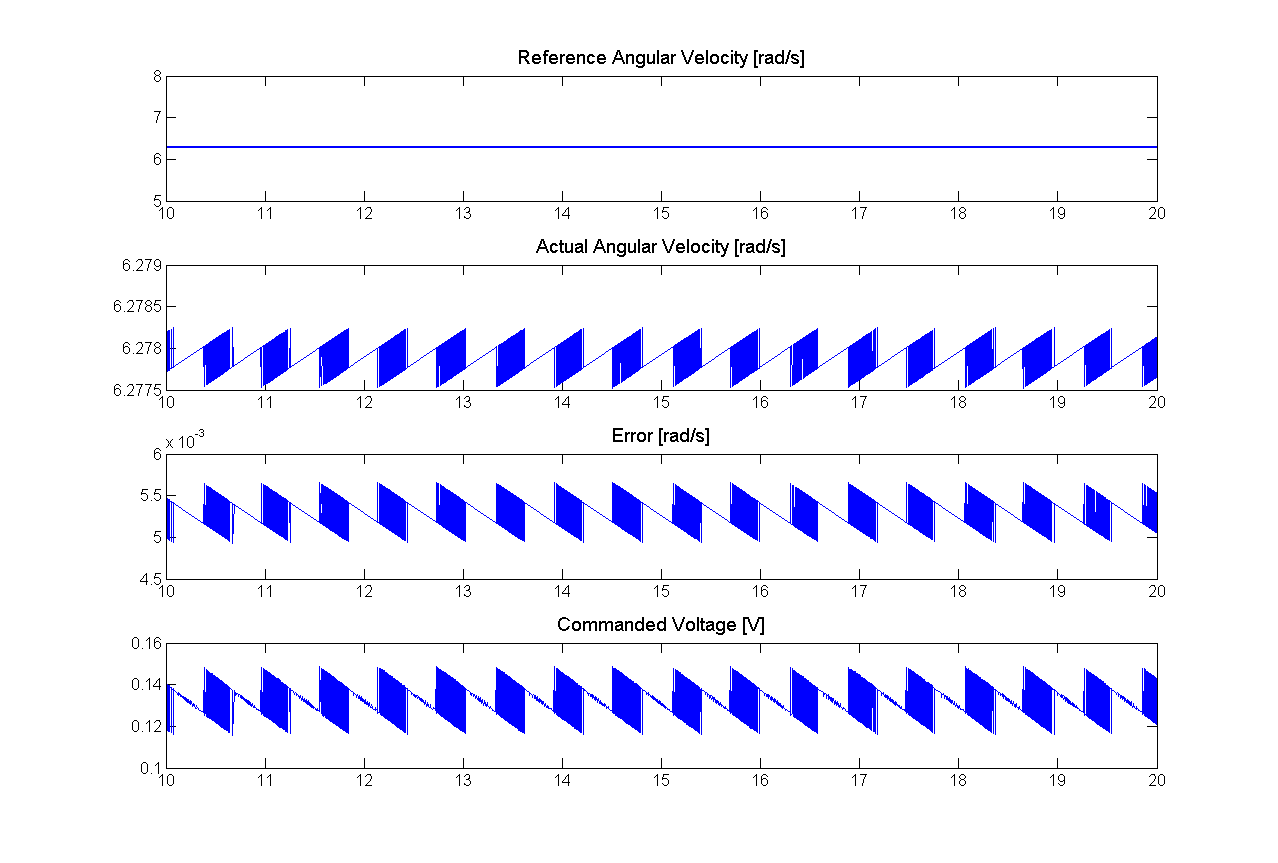
\includegraphics[width = 14 cm]{q3_12}
\caption{Step Command of 2$\pi$ radians/sec}
\label{q3_12}
\end{center}
\end{figure}

\begin{figure}[htb]
\begin{center}
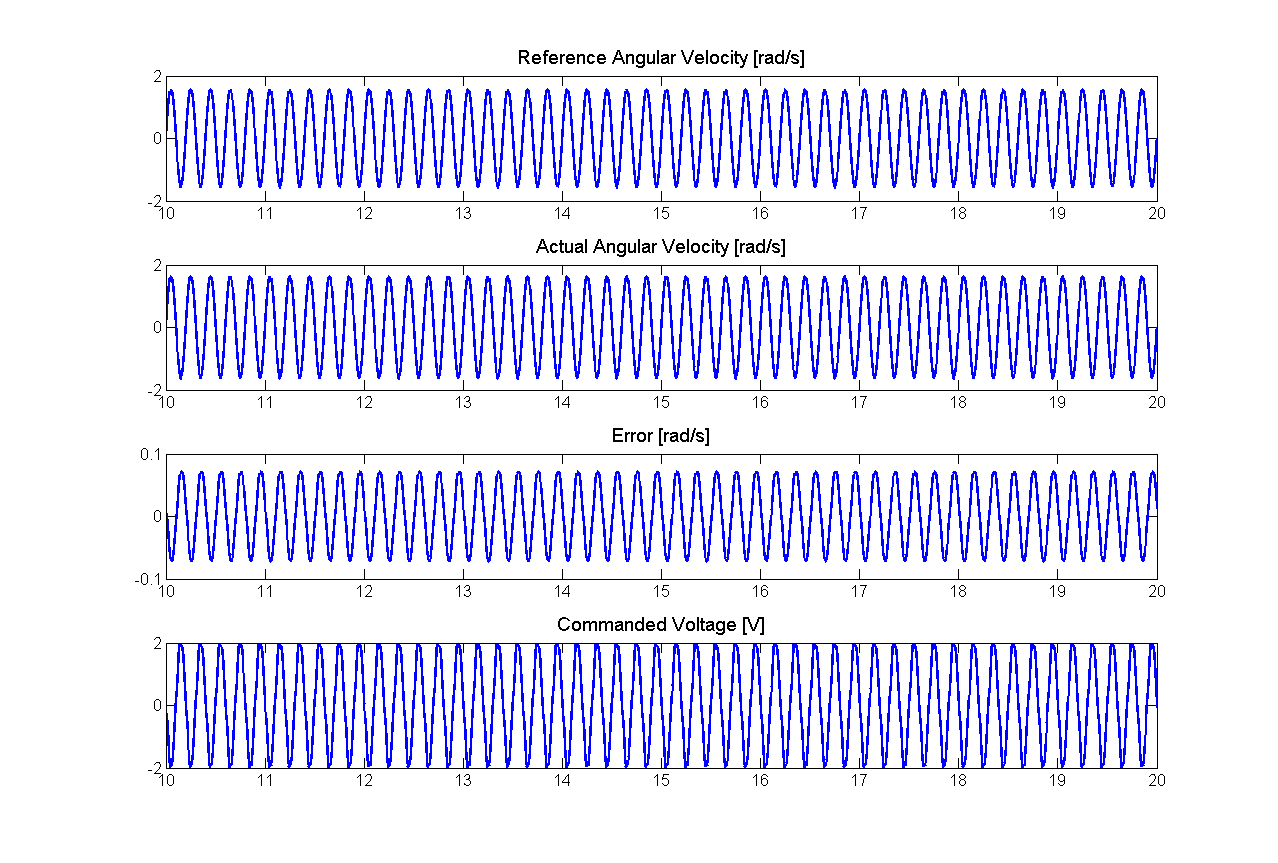
\includegraphics[width = 14 cm]{q3_13}
\caption{5Hz Sinusoidal Command of $\pi/2$ radians/sec}
\label{q3_13}
\end{center}
\end{figure}

\begin{figure}[htb]
\begin{center}
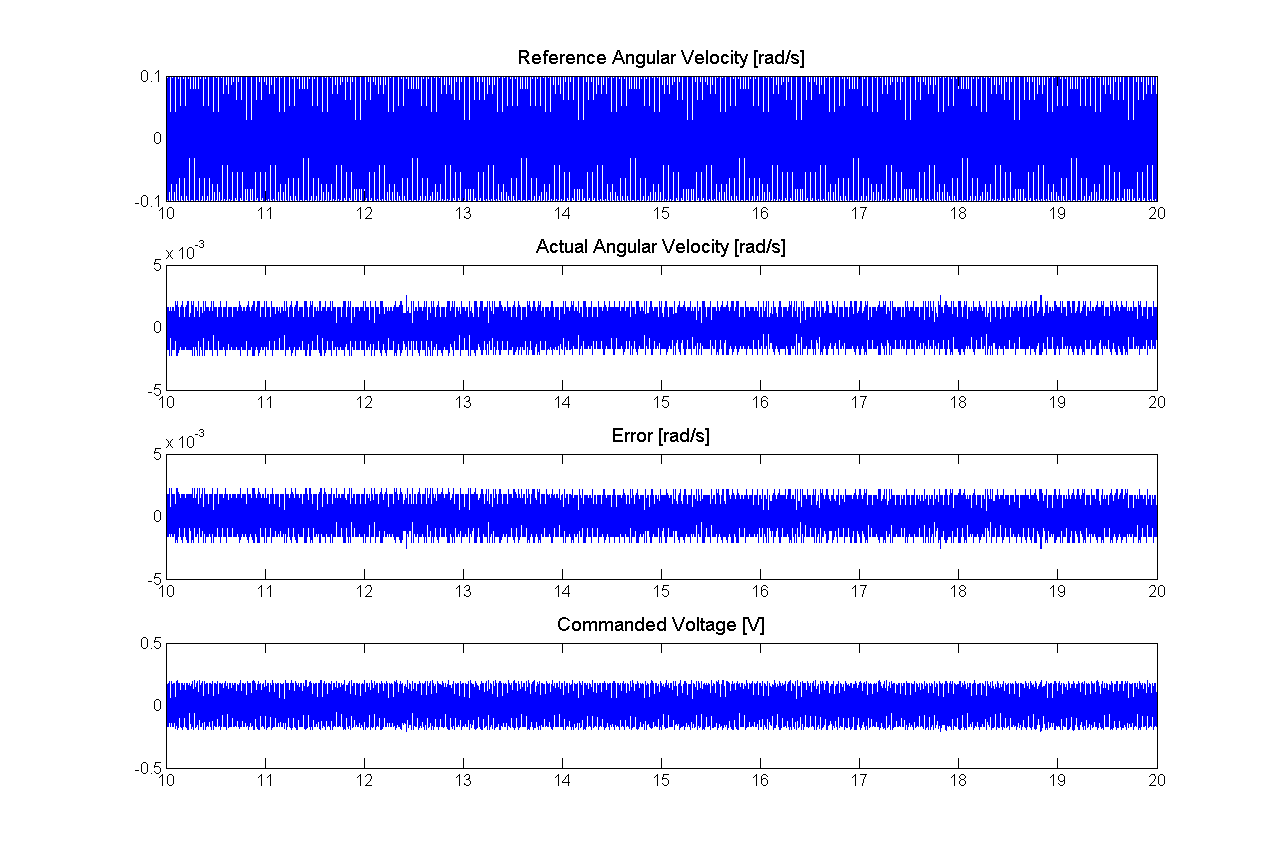
\includegraphics[width = 14 cm]{q3_14}
\caption{60Hz Input Disturbance of 0.1 radians/sec}
\label{q3_14}
\end{center}
\end{figure}

\begin{figure}[htb]
\begin{center}
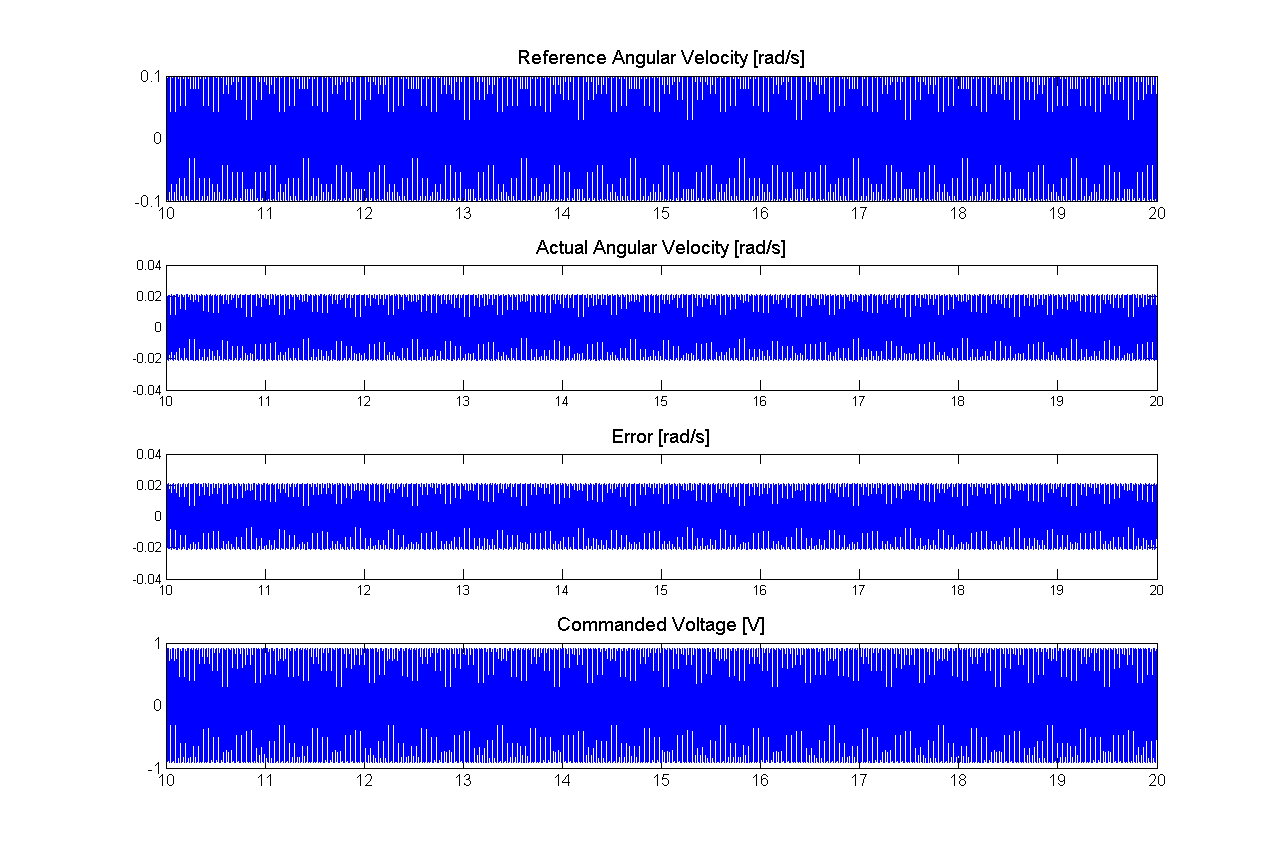
\includegraphics[width = 14 cm]{q3_15}
\caption{60Hz Output Disturbance of 0.1 radians/sec}
\label{q3_15}
\end{center}
\end{figure}




\clearpage

\subsection*{Position Control System - Dynamics Analysis}
As shown in figure \ref{q3_16}, there is steady-state error in the tracking function ($G_{CL}$) within the bandwidth. Furthermore, despite all frequencies below 0 dB for the transfer function of output disturbance rejection $G_{do}$, there is a peak around 60Hz which should be noticed. Both issues were critical to our objectives of control.

\begin{figure}[htb]
\begin{center}
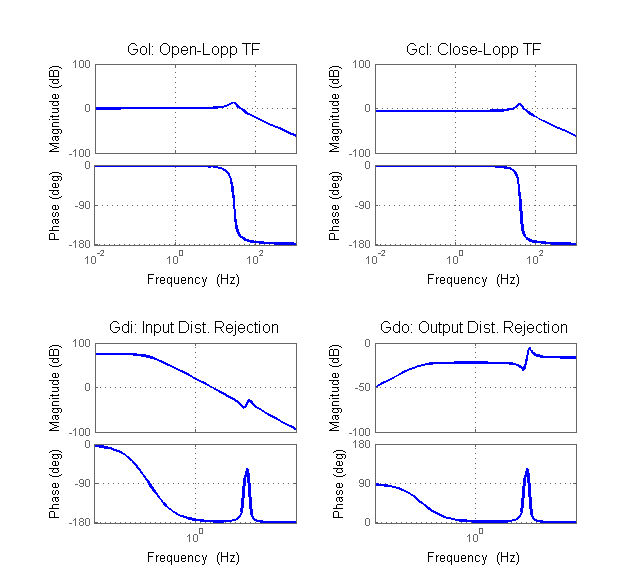
\includegraphics[width = 16 cm]{q3_16}
\caption{Bode Diagrams for the Transfer Functions of Open-Loop ($G_{POL}$), close-loop ($G_{PCL}$), input disturbance rejection ($G_{di}$), and output disturbance rejection ($G_{do}$) }
\label{q3_16}
\end{center}
\end{figure}

\clearpage

\subsection*{Position Control System – Controller Tuning}

$$K_{PP}: \text{Proportional Gain}$$
$$K_{PD}: \text{Derivative Gain}$$
$$K_{VF}: \text{Feedforward Gain}$$

\subsubsection*{a) Keep steady state error below 2\% for a step command of $\pi$ radians.}
\begin{itemize}
\item Setting $K_{PP}=1$, we see that the error did not fall below the required value. This is because if $K_{PP}$ was increased until the goal was attained, the commanded voltage exceeded the continuous current limit (2A).

\item In order to solve the problem, velocity feedforward control ($K_{VF}$) was introduced to provide better tracking performance without affecting the stability of the closed-loop system.

\item When $K_{VF} = 1$, the tracking error became nearly zero. 
\end{itemize}

\subsubsection*{b) Provide command tracking: Amplitude should remain within 5\% of commanded amplitude of pi radians, up until 5Hz.}
\begin{itemize}
\item With the identical setting, the tracking error of 5Hz command was close to zero as well.    
\end{itemize}


\subsubsection*{c) Attenuate a 60Hz noise signal coming in either at the servo-amplifier or the sensor by at least 10 times.}
\begin{itemize}
\item	A noise signal with amplitude 0.1 was used to test disturbance rejection. For the input disturbance (from servo amplifier), over 90\% was rejected; while none of the output disturbance (from the sensor) was rejected but at times, it was seen to even enlarge. 

\item The above situation was similar to that in the velocity control system, but $\tau$ was already tuned for the velocity loop. Therefore, we needed the derivative controller to improve the quality of disturbance rejection.  

\item Achieving all objectives simultaneously seemed to be impossible due to the limit on the commanded voltage (2A); in particular, the 60Hz noise was hardly  attenuated five times. Thus, we removed the quantizer to get a more favorable system. 

\item By trial and error, finally three objectives were achieved with $K_{PP}=2$,$K_{PD}=0.09 (N \footnote{Simulinks causality filter}=150)$,$K_{VF}=1$, and $\tau = 6.6$. However, the ability of output disturbance rejection was limited with amplitude 0.08. If the noise exceeded this limit, the commanded voltage would go beyond the current limit; that is, more power was required.     

\end{itemize}

\begin{figure}[htb]
\begin{center}
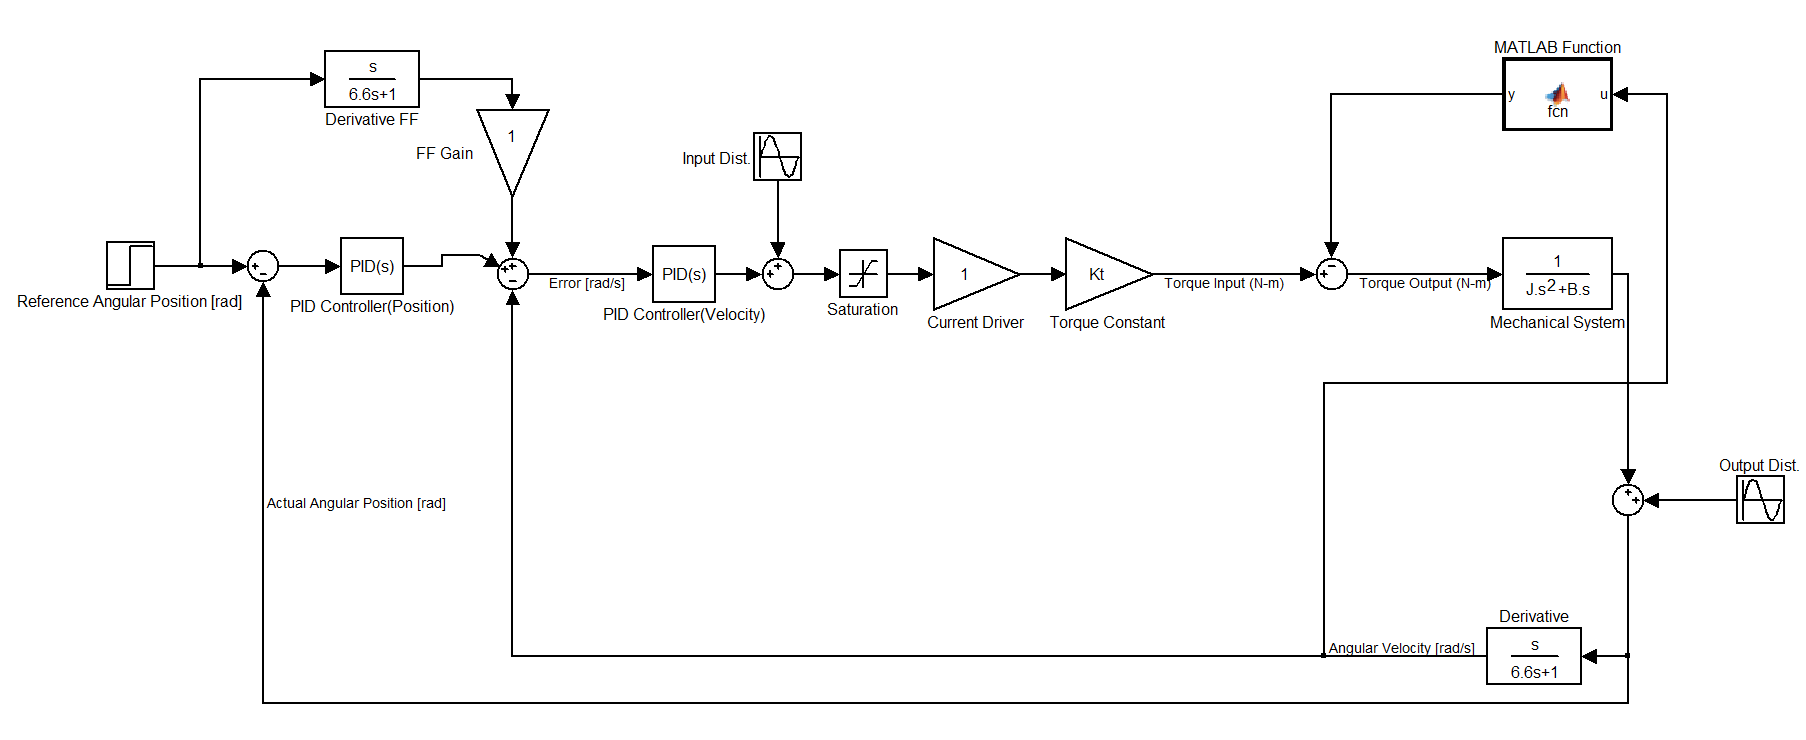
\includegraphics[height = 10cm, width = 16 cm]{q3_17}
\caption{Block Diagram of Position Control system}
\label{q3_17}
\end{center}
\end{figure}

\begin{table}[htb]
\begin{center}
    \begin{tabular}{|c|c|c|c|c|}
        \hline
        $K_{VF}$ & $K_{PP}$ & $K_{PD}$ & $N$ & $\tau$ \\ \hline
        1        & 2        & 0.09     & 150 & 6.6    \\
        \hline
    \end{tabular}
\caption{Controller Gains and $\tau$ of Position Control system}
\end{center}
\end{table}


\begin{table}
\begin{center}
    \begin{tabular}{|c|c|c|c|c|}
        \hline
        Reference               & Input Amplitude  & Output Amplitude  & \%Error & Commanded Voltage  \\ 
        ~                       & [rad]          & [rad]           & ~       & [Max. V]           \\ \hline
        (d) Step                & $\pi$              & 3.139             & 0.10\%  & 0.13               \\ 
        (e) Sinusoidal (5Hz)          & $\pi$              & 3.144             & 0.16\%  & 0.3                \\ 
        (f) Input Disturbance   & 0.1              & 0.002             & 2.02\%  & 1.55               \\ 
             Output Disturbance & 0.08             & 0.003             & 3.75\%  & 1.95               \\
        \hline
    \end{tabular}
\caption{Simulation Results for Different Reference Inputs}
\end{center}
\end{table}


Without a quantizer in the sensor, the three goals were achieved by similar tuning procedures. Due to the fact that position control was based on the velocity control, it seemed reasonable that the errors would be larger by combination if all settings were the same. Additionally, feedforward control was used in the position loop. It improved tracking performance and also eliminated the steady-state error for sinusoidal inputs, but it seemed have no effects on the velocity control.  

\begin{figure}[htb]
\begin{center}
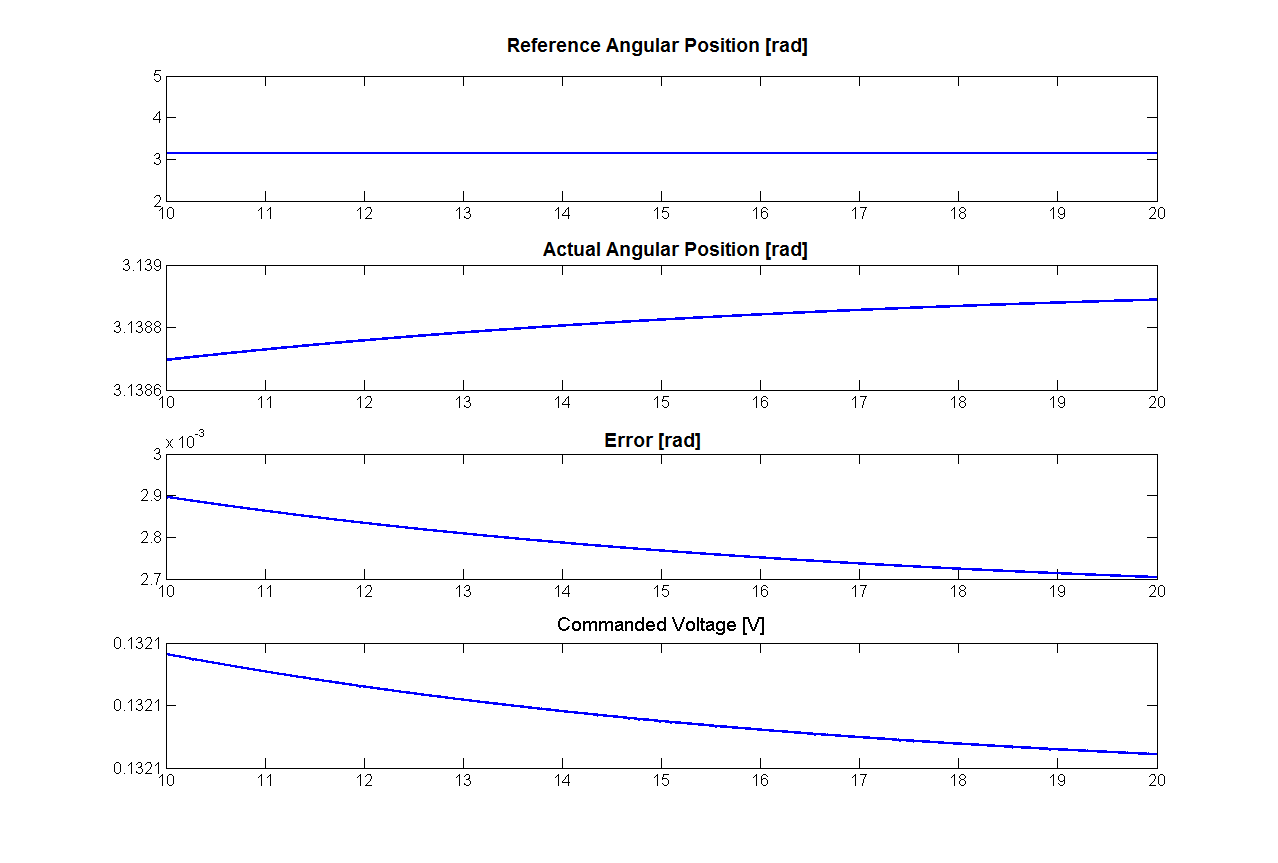
\includegraphics[width = 13 cm]{q3_18}
\caption{Step Command of $\pi$ radians}
\label{q3_18}
\end{center}
\end{figure}

\begin{figure}[htb]
\begin{center}
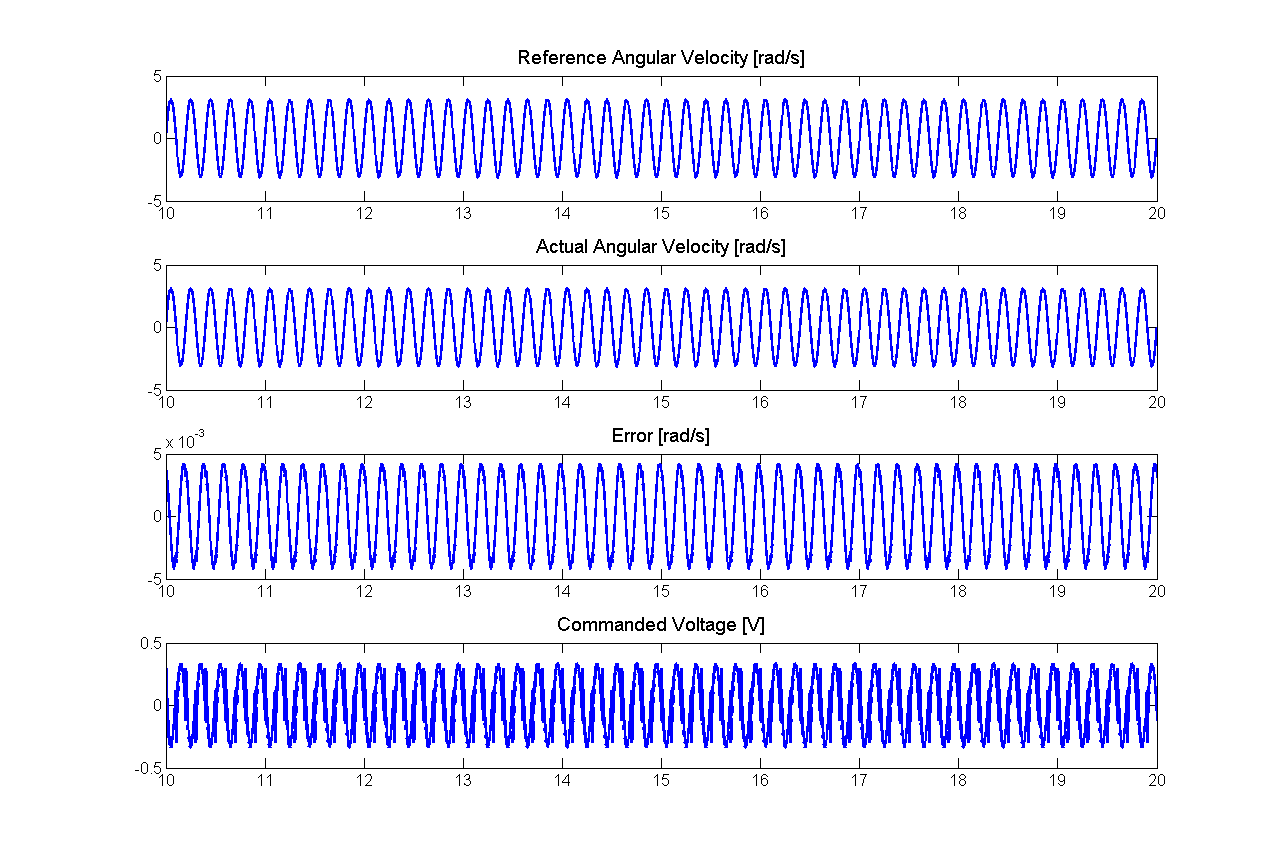
\includegraphics[width = 13 cm]{q3_19}
\caption{5Hz Sinusoidal Command of $\pi/2$ radians/sec}
\label{q3_19}
\end{center}
\end{figure}

\begin{figure}[htb]
\begin{center}
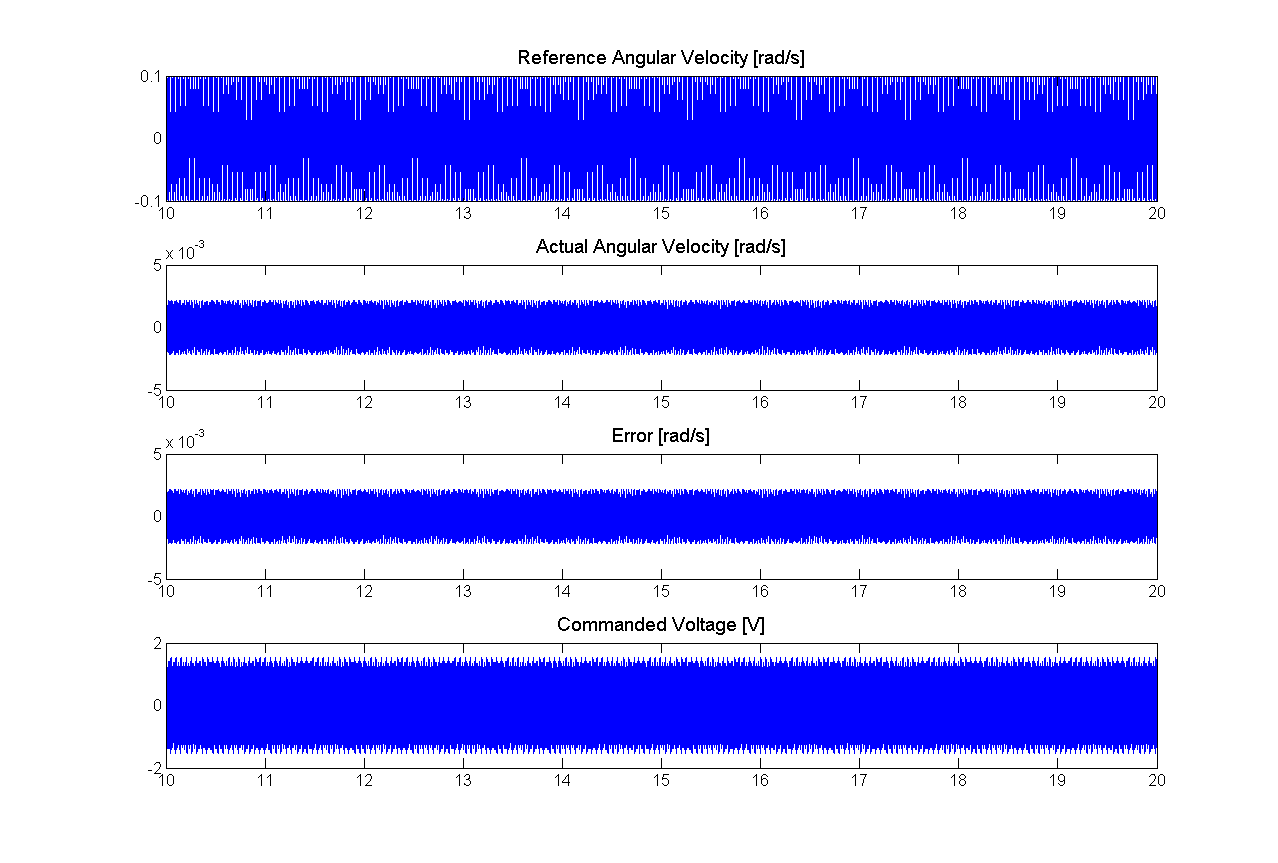
\includegraphics[width = 13 cm]{q3_20}
\caption{60Hz Input Disturbance of 0.1 radians}
\label{q3_18}
\end{center}
\end{figure}

\begin{figure}[htb]
\begin{center}
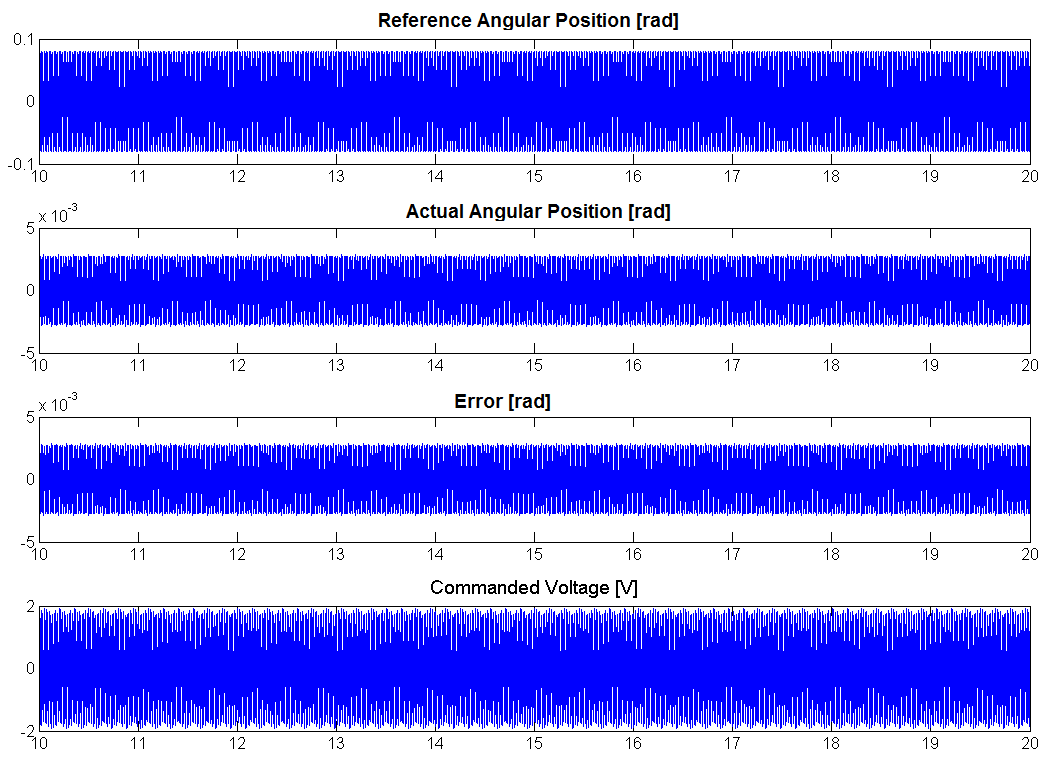
\includegraphics[width = 13 cm]{q3_21}
\caption{60Hz Output Disturbance of 0.1 radians}
\label{q3_21}
\end{center}
\end{figure}

\clearpage

\section*{4.}

\subsection*{a.}
When we implemented the controller and values from our simulation in part 3, we were unable to achieve stable output in the physical system. Therefore, we kept the same general approach - a velocity controller nested within a position controller with feed forward - but we re-tuned the system with different gain values. Because we have a velocity controller inside of our position controller, we first tuned the velocity control on its own (see section 6). Once it was working, we then implemented it in the inner loop of our position controller and tuned the position control gains. In the end we were not able to meet all of the control goals with one controller. We designed one controller with good step response and noise attenuation, and then modified the gain values to improve the frequency response separately. The results for the step response and noise attenuation are given below.\\


\begin{table}[htb]
\begin{center}
    \begin{tabular}{|c|c|c|c|c|c|}
        \hline
        Gains & P   & I & D   & Feed Forward   & Filter $\tau$   \\ \hline
        Position Loop            & 0.1 & 20  & 0 & 1 & 6.5797    \\ 
        Velocity Loop       & 22.5   & 22.5    & 1.125   & -  & 6.5797  \\ 
       \hline
    \end{tabular}
\end{center}
\caption{Values of position controller with nested velocity controller for step response and noise attenuation}
\label{positionGains}
\end{table}

Figure \ref{PosStepPi} shows the system's response to a position step input of $\pi$ radians, and figure \ref{PosStepError} shows a zoomed in view after it had settled. The peak error here is 0.11\%, which out performs the goal of 2\% error. Additional results for position steps of different magnitudes are included in section 5b.  The error seen here is very similar to the steady state error of 0.10\% predicted in our simulink simulation in response to a step input of $\pi$ radians.\\

\begin{figure}[htb]
\begin{center}
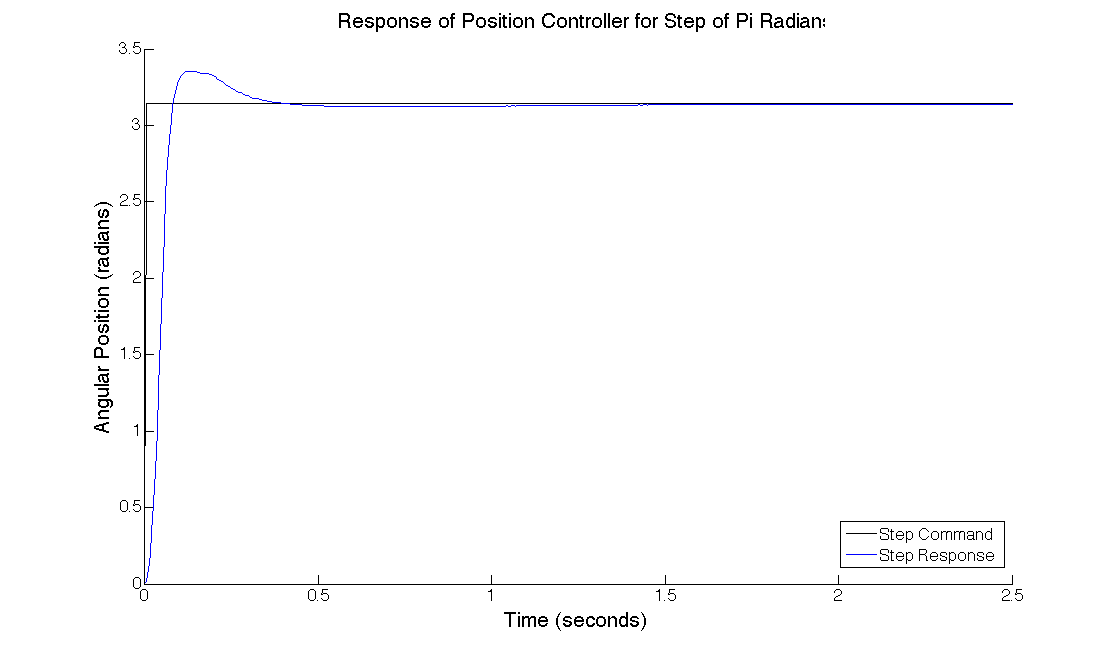
\includegraphics[width = 14cm]{posstep_1pi.png}
\caption{Step response of position controller}
\label{PosStepPi}
\end{center}
\end{figure}

\begin{figure}[htb]
\begin{center}
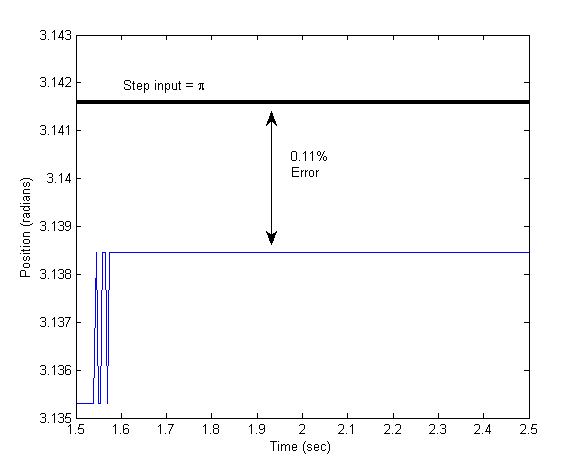
\includegraphics[width = 12cm]{positionStepError.png}
\caption{Steady state error for position step input of $\pi$}
\label{PosStepError}
\end{center}
\end{figure}

Figure \ref{PosNoise} shows the noise attenuation during a step input of $\pi$ radians. To simulate the noise within LabView, we added a 60 Hz sine signal with an amplitude of 1 to the output of the DAQ assistant. Figure \ref{PosNoiseZoom} shows a zoomed in view after the step has taken place. For the step response with no noise, our steady state error was approximately 0.003, and with the noise the highest error is 0.060. Given that we were inputting a noise amplitude of one and the error only increased by 0.057, we have attenuated the noise by approximately 17.54 times. This exceeds the goal of a ten times reduction.\\

\begin{figure}[htb]
\begin{center}
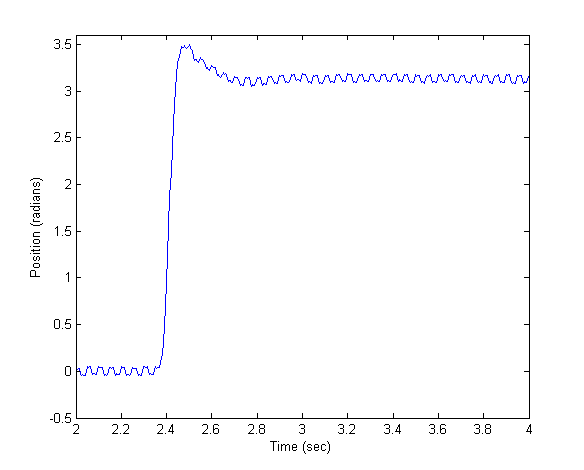
\includegraphics[width = 12cm]{PosNoise.png}
\caption{Step response for input of $\pi$ with a 60 Hz noise signal (amplitude = 1)}
\label{PosNoise}
\end{center}
\end{figure}

\begin{figure}[htb]
\begin{center}
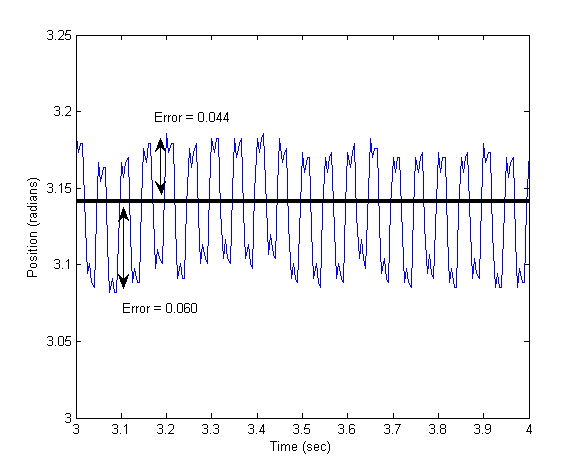
\includegraphics[width = 12cm]{PosNoiseZoom.png}
\caption{Steady state step response for input of $\pi$ with a 60 Hz noise signal (amplitude = 1)}
\label{PosNoiseZoom}
\end{center}
\end{figure}

The position controller we were using for the step response and noise attenuation did not not perform well with sinusoidal inputs forcing us to modify gains while keeping the overall architecture the same. The relevant values are given in the table \ref{positionFreqGains}, and the following figures show the response at various frequencies with an amplitude of $\pi$. Figure \ref{PosFreqError} shows the error as a function of input frequency. During our tests the position output remained stable up to 5 Hz, but the output amplitude error exceeded 5\% just beyond 4 Hz. This does not meet the goal of less than 5\% error up to 5 Hz.  The performance of the real system at 5 Hz with an output magnitude of -2.078 dB performs far worse than our simulated system which maintained a 0 dB magnitude at the same frequency \\

\begin{table}[htb]
\begin{center}
    \begin{tabular}{|c|c|c|c|c|c|}
        \hline
        Gains & P   & I & D   & Feed Forward   & Filter $\tau$   \\ \hline
        Position Loop            & 0 & 20  & 0 & 1 & 6.5797    \\ 
        Velocity Loop       & 3   & 7    & 0.4   & -  & 6.5797  \\ 
       \hline
    \end{tabular}
\end{center}
\caption{Values of position controller with nested velocity controller for frequency response}
\label{positionFreqGains}
\end{table}

\begin{table}[htb]
    \begin{tabular}{|c|c|c|c|c|}
        \hline
        Frequency (Hz) & Input Amplitude & Output Amplitude & Magnitude (dB) & \%Error       \\ \hline
        1              & $\pi$           & 3.13845          & -0.008693172   & -0.100033771 \\ 
        2              & $\pi$           & 3.02221          & -0.336504689   & -3.800067888 \\ 
        3              & $\pi$           & 3.079209         & -0.174214105   & -1.985733367 \\ 
        4              & $\pi$           & 3.030152         & -0.313709167   & -3.547266176 \\ 
        5              & $\pi$           & 2.473084         & -2.078220099   & -21.27929134 \\ 
        5.27           & $\pi$           & 2.181877         & -3.166392169   & -30.54869805 \\
        \hline
    \end{tabular}
    \caption{Position control data.}
    \label{q4_atable}
\end{table}

\begin{figure}[htb]
\begin{center}
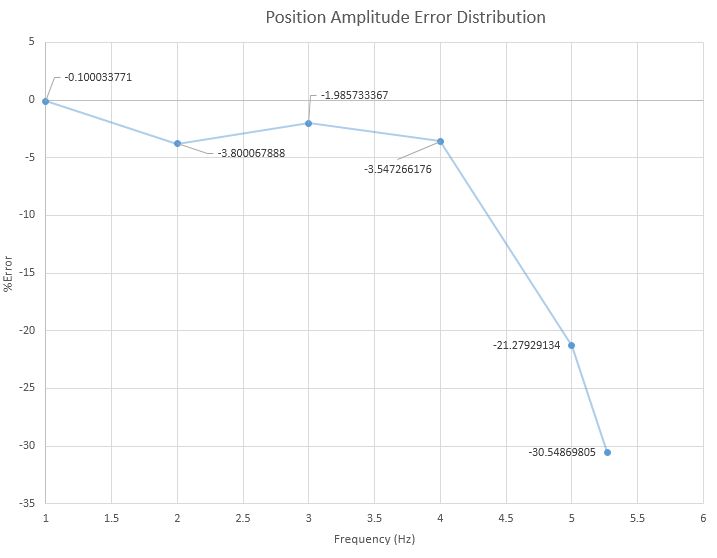
\includegraphics[width = 14cm]{PositionControl_Error.png}
\caption{Position error vs. frequency for an input amplitude of $\pi$ radians}
\label{PosFreqError}
\end{center}
\end{figure}

To determine the closed-loop bandwidth of the system, we slowly increased the frequency of the input signal until the output amplitude just crossed -3 dB (for a input of $\pi$ this corresponded to an output of 2.22). We found that the bandwidth of our position control system was 5.27 Hz, as shown in figure \ref{PosBandwidth}.\\

\begin{figure}[htb]
\begin{center}
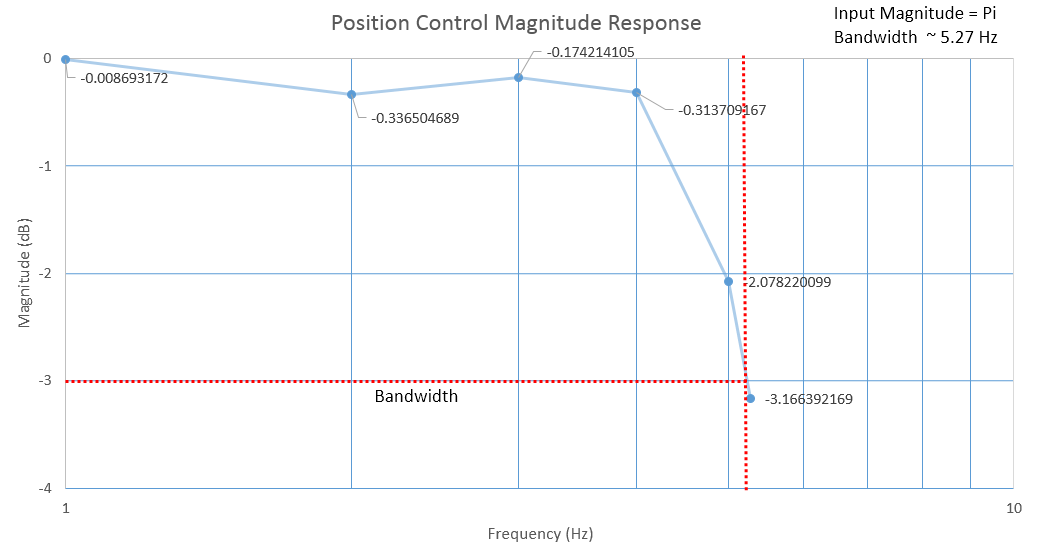
\includegraphics[width = 14cm]{PositionControl_Magnitude.png}
\caption{Output magnitude vs. frequency used to determine bandwidth of position controller}
\label{PosBandwidth}
\end{center}
\end{figure}

Even though we included many nonlinear factors in our simulation, we still faced difficulties meeting all of the performance specifications, particularly trying to do so with just one controller. In general, we found that when we adjusted gains to meet the step requirement, the frequency response usually got worse, and vice-versa. It's possible that some of the values used in our simulation are incorrect (even after testing and regression), or that there are other factors we did not account for, such as the dynamics of the servo-amp. In the end we were able to meet the steady state error for step input and noise attenuation requirements, and were very close to the frequency response requirement.\\


\clearpage 

\section*{5.}
\subsection*{ Comparison of Our System Model with the Data Sheet and the Physical System}
\begin{table}[htb]
    \begin{tabular}{|c|c|c|c|c|}
        \hline
        ~                        & Original Model & Original Model   & New Model & Real Physical System \\ 
	~	& ~	& (with gains used in VI)& (with gains used in VI)& ~\\ \hline
        BW of Velocity Loop [Hz] & 6.52           & 6.52                                    & 2.8                               & 2.9                  \\ 
	~&	~&	~&	~&	~\\
        BW of Position Loop [Hz] & 11.4           & 11.8                                    & 5.1                    & 5.27     \\
	~ &~	&~	&\emph{(with I =1)} & \emph{(with I =10)}\\
        \hline
    \end{tabular}
\end{table}

The original model was built using the values of $J, b$ and $\tau_f$ and optimized to provide the best performance. We then proceeded to measure the actual system parameters empirically. Using the measured values as well as accounting for non-linear effects like saturation and varying friction, we made a second model - the new model. At the same time we proceeded to tune the physical system. We then incorporated the practical values used in the real system on our theoretical system for comparison of how well our model simulates the real world. As you can see from the table above, our model does a very realistic job of modeling the system.

\begin{figure}[htb]
\begin{center}
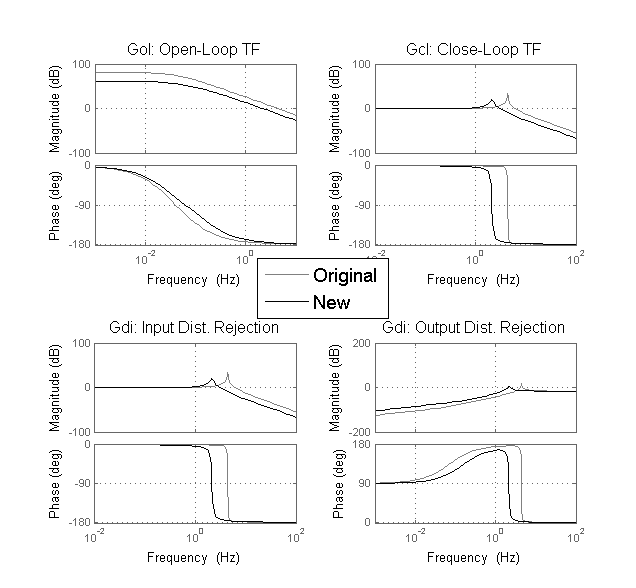
\includegraphics[width = 13.5cm]{Original_vsNew.png}
\caption{Comparison of the new model with the original model.}
\label{q5_orig_v_new}
\end{center}
\end{figure}

\clearpage

\subsection*{a. Coulomb Friction}
The bearings in the motor are the primary source of coulomb friction in the motor encoder system. This could be especially true in the current configuration of the motor because Pittman's website only specifies that they use ball or sleeve bearings in their products. If these are only radial bearings with no thrust capability, then the motor's performance could be affected by the vertical mounting we are using. Additionally, there is friction between the brushes and commutator. In section 2b we discussed and carried out experiments and modeling to determine the friction value.\\

Setting aside the earlier parameter identification, there are some simple experiments that could be run to estimate the friction in the system. If we assume that the torque constant given in the data-sheet is correct and that the gain of the servo-amp is exact and known, then for a given command voltage, the motor should be capable of a specific torque output. By slowly increasing the voltage from zero until the motor just begins to turn. From this, the torque caused by static friction would be equal to the product of the torque constant and the input voltage (because there is a 1:1 relationship between command voltage and applied current). \\

A similar method could be used to determine sliding friction. By applying a constant voltage to the system, the motor would come to a steady-state velocity. If we the coefficient of damping is known, then the torque caused by sliding friction is equal to the motor torque ($K_{t}$ * $V_{command}$) minus the torque from damping (the product of the damping coefficient and velocity). This was carried out in part 2b.\\

Friction was included in our Simulink model from the beginning of our modeling, as presented in part 3. At the beginning of our tests we used approximations based on the data-sheet values, but as we performed more regression analysis, we obtained new values that should be closer to the true values of the physical system. \\

\subsection*{b. Saturation}

Position Saturation\\

In the actual system, the effects of saturation can clearly be seen in the steady increase of rise time as well as the decreasing stability of the system reflected in the higher percent overshoot and larger steady state error.  With saturation, the system is not able to move at the speed at which the controller requests, meaning that rise time will become dependent on the actual input magnitude, rather than being independent as is normally the case without saturation.  The loss of stability that we see is an effect of integral wind up.  Because the system takes longer to respond, our integral term has a longer period of time to accumulate error, which then has to be canceled out with positive error, leading to large overshoots and long settling times.  In extreme cases this can drive the system to instability.  The effects of saturation on integrator wind up can be compensated for by limiting the maximum and minimum values that the integrator can accumulate.  Another method is to model the saturation effect and use this model to alter the input to the integrator such that when the driver becomes saturated, the integrator no longer receives input. \\

As can be seen in figure \ref{q5_b0} our model also exhibits the same large rise time that we would expect for extremely large input signals.  

\begin{table}[htb]
\begin{center}
    \begin{tabular}{|c|c|c|c|c|c|}
        \hline
        Step Input Amplitude (Radians) & $1\pi$   & $1.5 \pi$ & $2\pi$   & $3\pi$   & $4\pi$   \\ \hline
        Rise Time (seconds)            & 0.0700002 & 0.0800000   & 0.0850000 & 0.110000 & 0.125    \\ 
        Settling Time (seconds)        & 0.290000   & 0.320000    & 0.28000   & 0.54500  & 1.45500  \\ 
        Percent Overshoot (\%)          & 6.79997   & 16.8000     & 31.8500   & 65.0331  & 91.0003  \\ 
        Steady State Error (\%)         & 0.100034  & 0.594022    & 0.150008  & 0.13335  & 0.399713 \\
        \hline
    \end{tabular}
\end{center}
\caption{Step Response for a variety of input positions.  Where rise time is defined as reaching 90\% of the final value while settling time is the time after which the function remains within 2\% of its final value}
\label{q5_b6}
\end{table}

\begin{figure}[htb]
\begin{center}
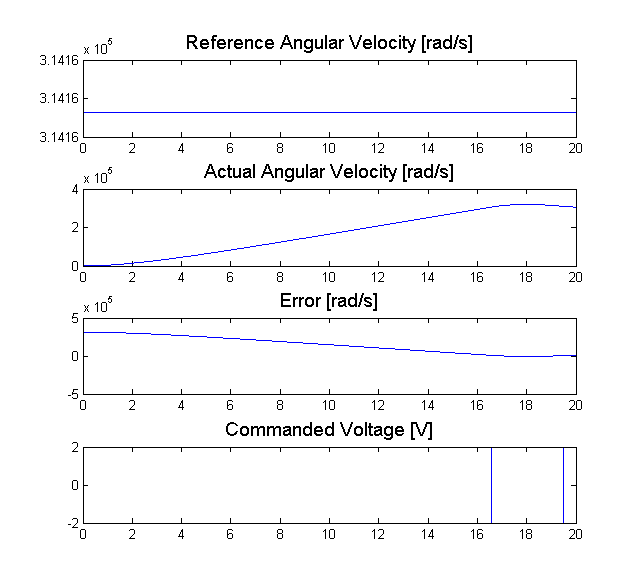
\includegraphics[width = 16cm]{q5b.png}
\caption{Tracking Ability for Extremely Large amplitude of step command}
\label{q5_b0}
\end{center}
\end{figure}
%^Alex's stuff



\begin{figure}[htb]
\begin{center}
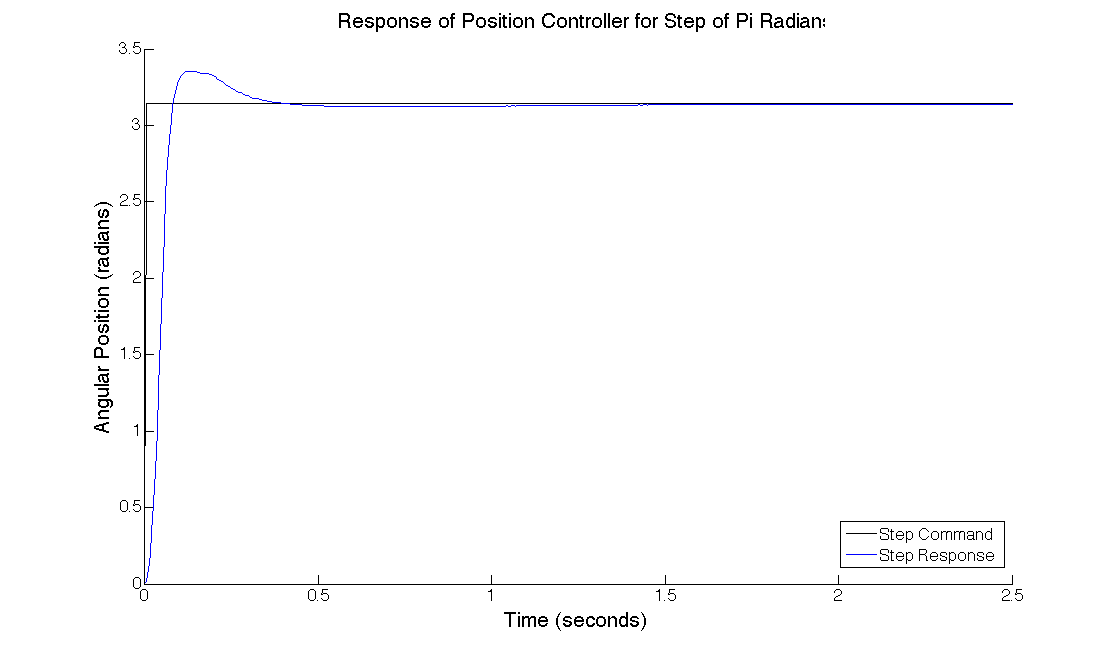
\includegraphics[width = 14cm]{posstep_1pi.png}
\caption{Step response of position controller}
\label{q5_b1}
\end{center}
\end{figure}

\begin{figure}[htb]
\begin{center}
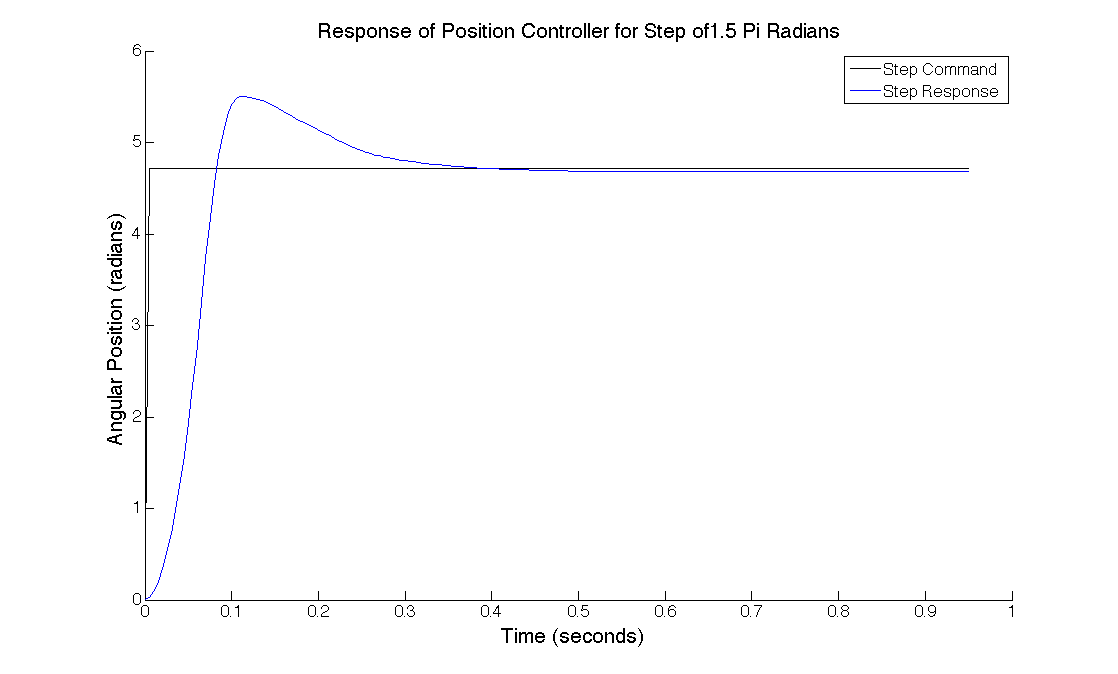
\includegraphics[width = 14cm]{posstep_15pi.png}
\caption{Step response of position controller}
\label{q5_b2}
\end{center}
\end{figure}

\begin{figure}[htb]
\begin{center}
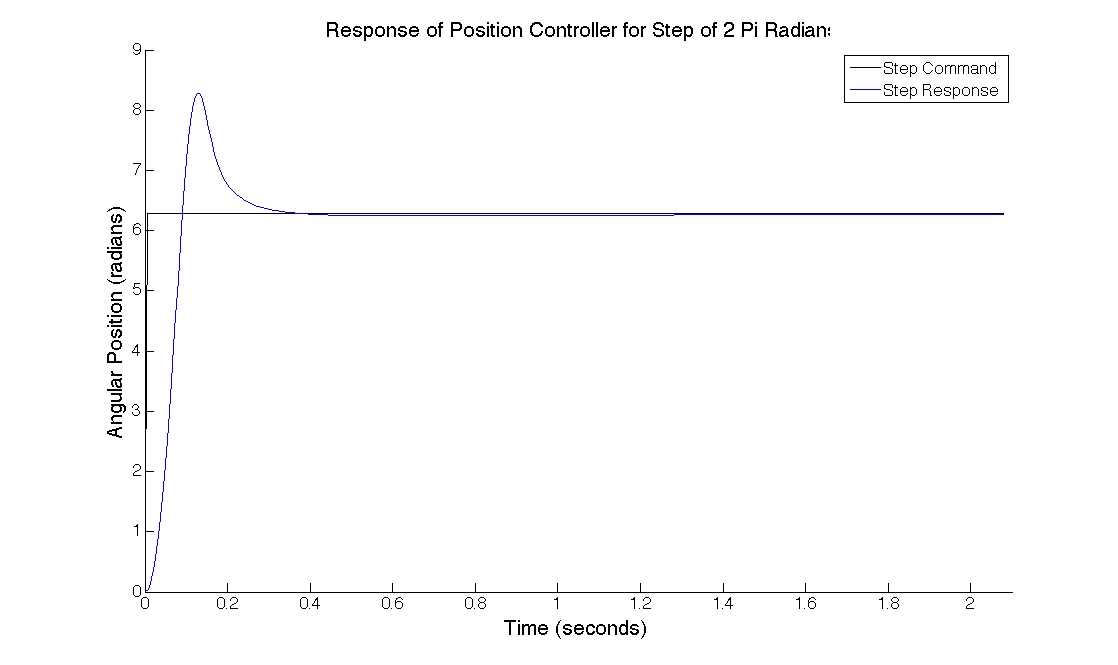
\includegraphics[width = 14cm]{posstep_2pi.png}
\caption{Step response of position controller}
\label{q5_b3}
\end{center}
\end{figure}

\begin{figure}[htb]
\begin{center}
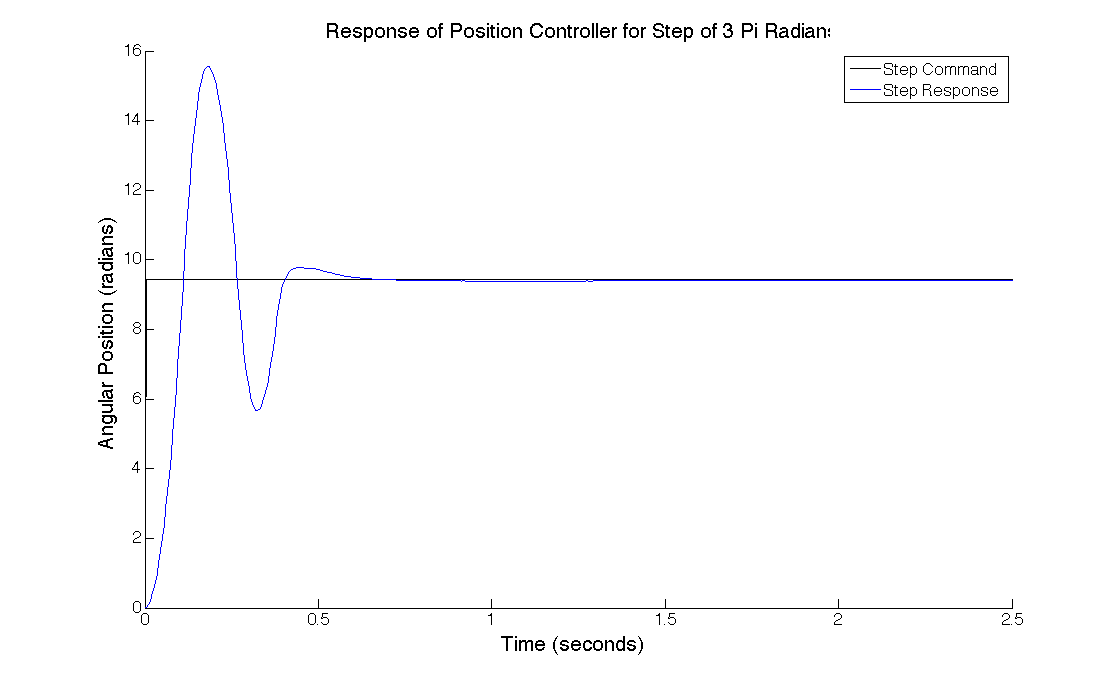
\includegraphics[width = 14cm]{posstep_3pi.png}
\caption{Step response of position controller}
\label{q5_b4}
\end{center}
\end{figure}

\begin{figure}[htb]
\begin{center}
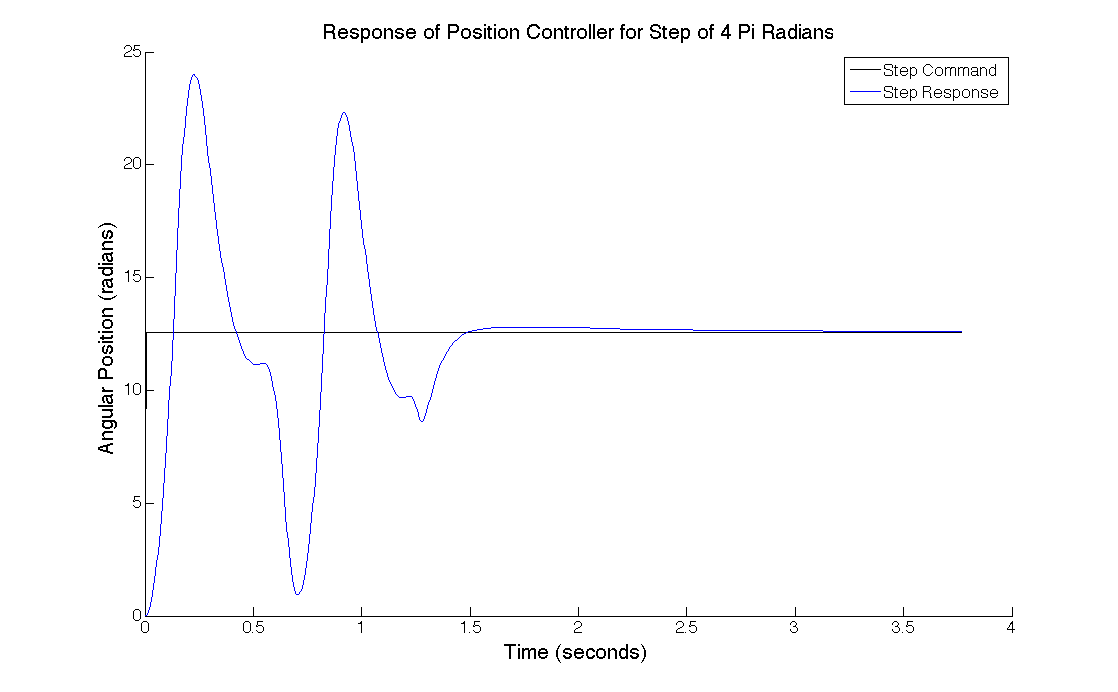
\includegraphics[width = 14cm]{posstep_4pi.png}
\caption{Step response of position controller}
\label{q5_b5}
\end{center}
\end{figure}

\clearpage

\subsection*{c. Quantization}
The real behavior of the optical encoder was already modeled as the quantizer with an interval $2\pi/2000$ in our model. The higher resolution of the sensor, the closer the system is to a  linear unity gain block, providing less measured error. The tracking error of sinusoidal input exceeded 5\% as the resolution reached 75 step/rev, while the error of step input went beyond 2\% when the resolution neared 325 steps/rev. \\

Most parasitic effects have been considered for our model. For quantization, we find it causes significant trouble in our position control. In feedback control systems, the sum of loop sensitivity  and complementary sensibility is one. Since the sensed error which resulted from quantization is based on the complementary sensitivity, more power is required to achieve the same closed-loop response; otherwise, the tracking error cannot be lowered in a desired manner. 

\begin{figure}[htb]
\begin{center}
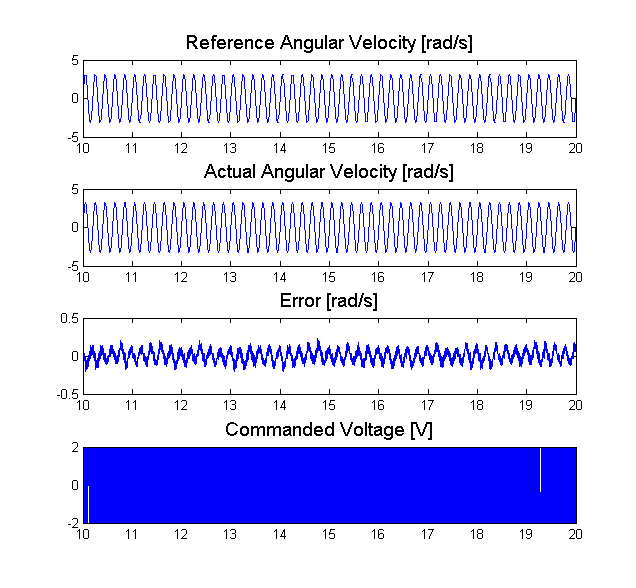
\includegraphics[width = 14cm]{q5c_sine_75.png}
\caption{Sinusoidal Tracking Error > 5\% when Resolution = 75 steps/rev}
\label{q5_c1}
\end{center}
\end{figure}
%^Alex's stuff

\begin{figure}[htb]
\begin{center}
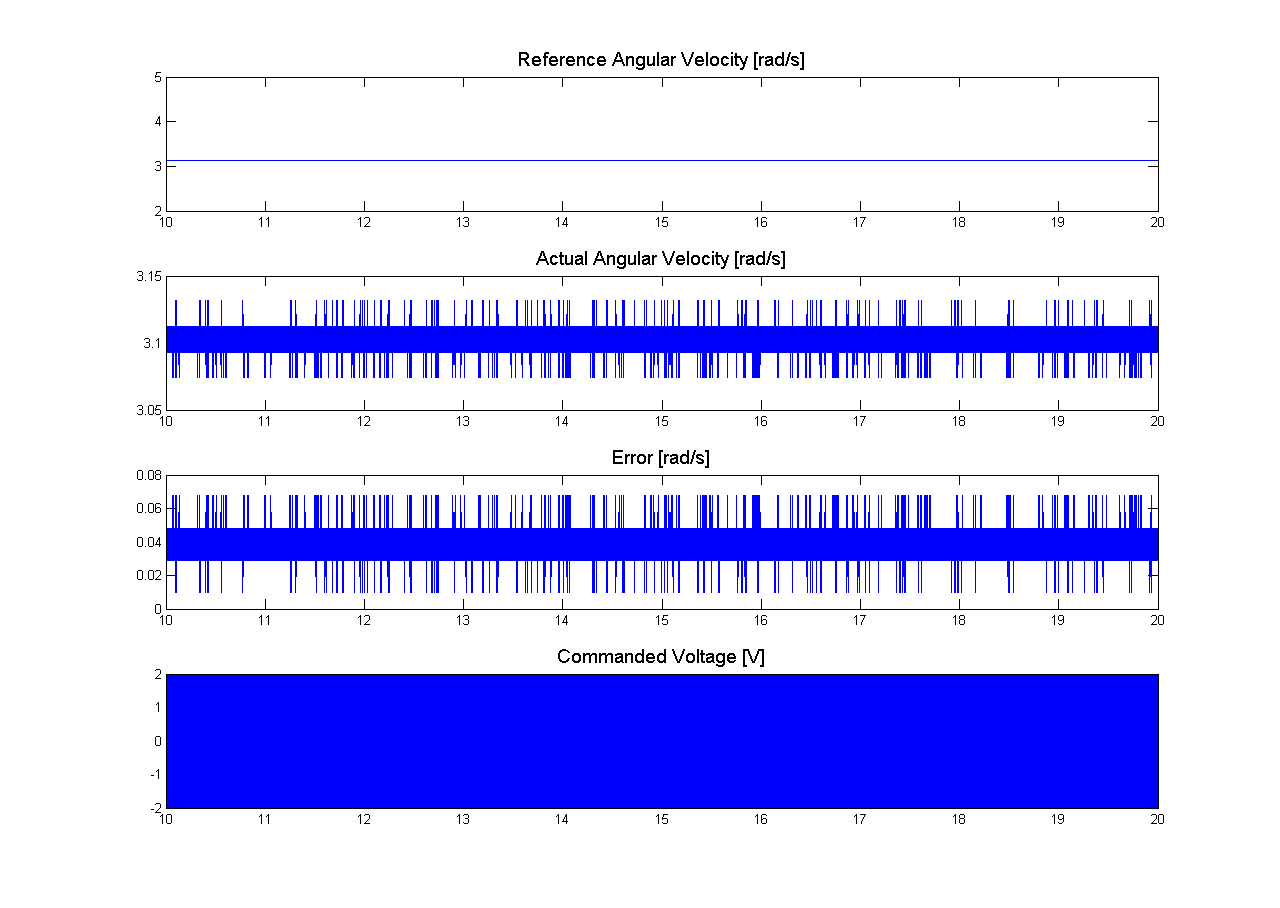
\includegraphics[width = 14cm]{q5c_step_325.png}
\caption{Step Tracking Error > 2\% when Resolution = 325 steps/rev}
\label{q5_c2}
\end{center}
\end{figure}
%^Alex's stuff


\clearpage

\section*{6.}
As was discussed in section 4, work on the velocity controller for the real system was performed before the position controller, because we needed to nest the velocity loop within the position loop. The gains we used in the simulation were not able to stabilize the system with the performance we wanted, so we re-tuned the gain values. As with position control, we were not able to use one controller to meet all of the requirements: we designed one controller that could meet the step and noise requirements, and then modified the gain values to improve the frequency response separately. The results for the step response and noise attenuation are given below. The gains used here are the same as in the step position controller's nested velocity loop.\\

\begin{table}[htb]
\begin{center}
    \begin{tabular}{|c|c|c|c|c|}
        \hline
        Gains & P   & I & D     & Filter $\tau$   \\ \hline
        Velocity Controller       & 22.5   & 22.5    & 1.125    & 6.5797  \\ 
       \hline
    \end{tabular}
\end{center}
\caption{Values of velocity controller for step response and noise attenuation}
\label{velocityGains}
\end{table}

Figure \ref{q6_4} shows the system's response to a velocity step input of 2$\cdot\pi$ radians, and figure \ref{VelStepError} shows a zoomed in view after it had settled. The peak error here is approximately 0.16\% (and on average is much less), which greatly exceeds the goal of 2\% error. Additional results for velocity steps of different magnitudes are also shown in the following tables and figures.\\

\xxx{Compare to simulation results}

\begin{figure}[htb]
\begin{center}
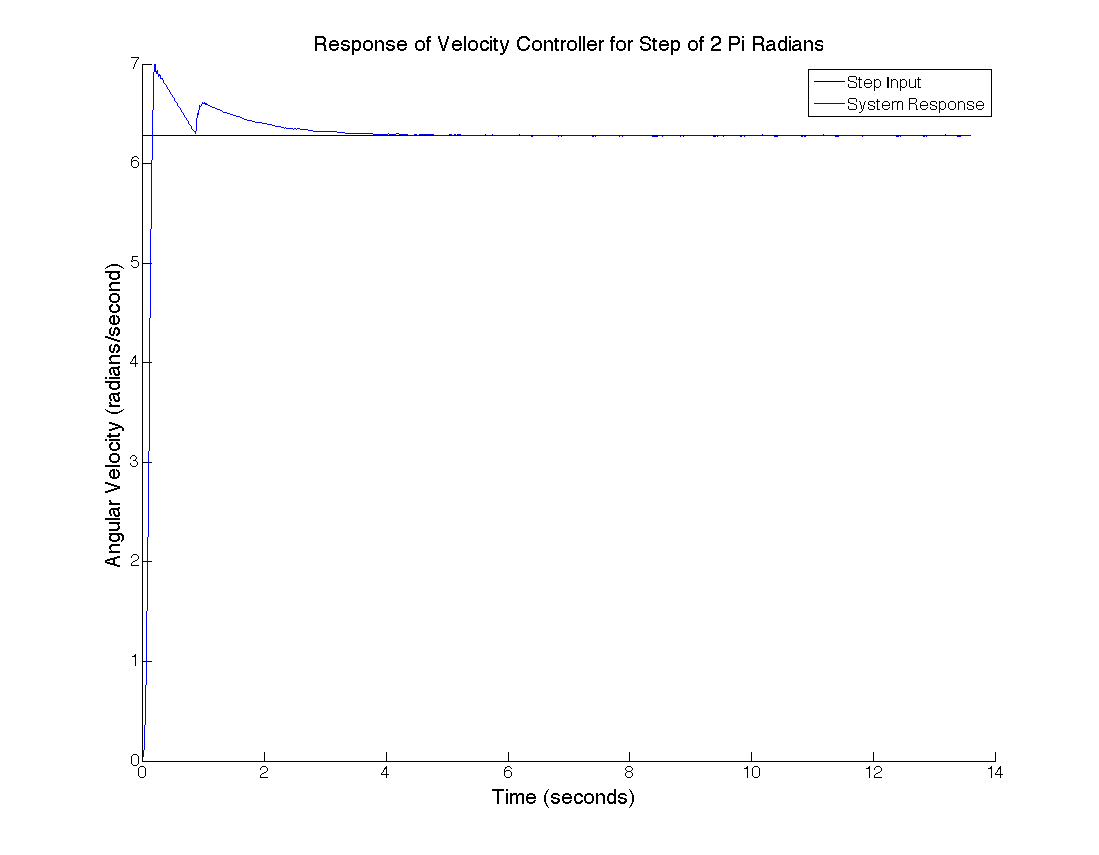
\includegraphics[width = 12cm]{velstep2Pi.png}
\caption{Velocity Controller Step Response}
\label{q6_4}
\end{center}
\end{figure}

\begin{figure}[htb]
\begin{center}
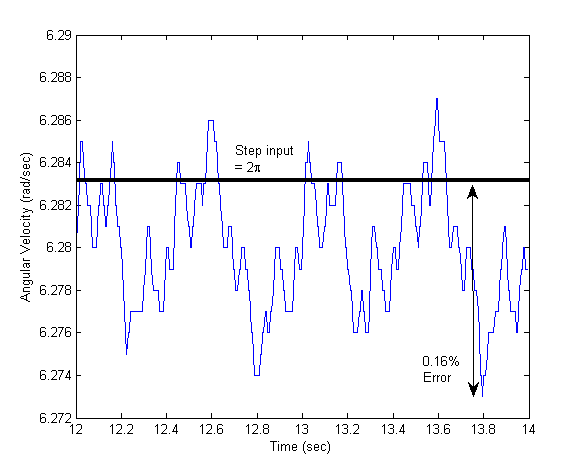
\includegraphics[width = 12cm]{VelStepError.png}
\caption{Steady state error for step input of 2$\cdot\pi$ rad/sec}
\label{VelStepError}
\end{center}
\end{figure}

\begin{table}[htb]
\begin{center}
    \begin{tabular}{|c|c|c|c|c|c|c|}
        \hline
        Step Input Amplitude (Radians) & $0.5 \cdot \pi$ & $1 \cdot \pi$ & $1.5 \cdot \pi$ & $2 \cdot \pi$ & $5 \cdot \pi$ & $10 \cdot \pi$ \\ \hline
        Rise Time (seconds)            & 0.11            & 0.115         & 0.125           & 0.14          & 0.23          & 0.385          \\ 
        Settling Time (seconds)        & 1.5700          &1.6700          & 1.95500           & 1.9700        & 2.3050        & 2.8550         \\ 
        Percent Overshoot (\%)         & 4.3415          & 6.1564        & 7.9919          & 11.3925       & 21.091        & 27.1553        \\ 
        Steady State Error (\%)        & 0.11779         & 0.041862      & 0.053597        & 0.058333      & 0.050267      & 0.050634       \\
        \hline
    \end{tabular}
\end{center}
\end{table}

\begin{figure}[htb]
\begin{center}
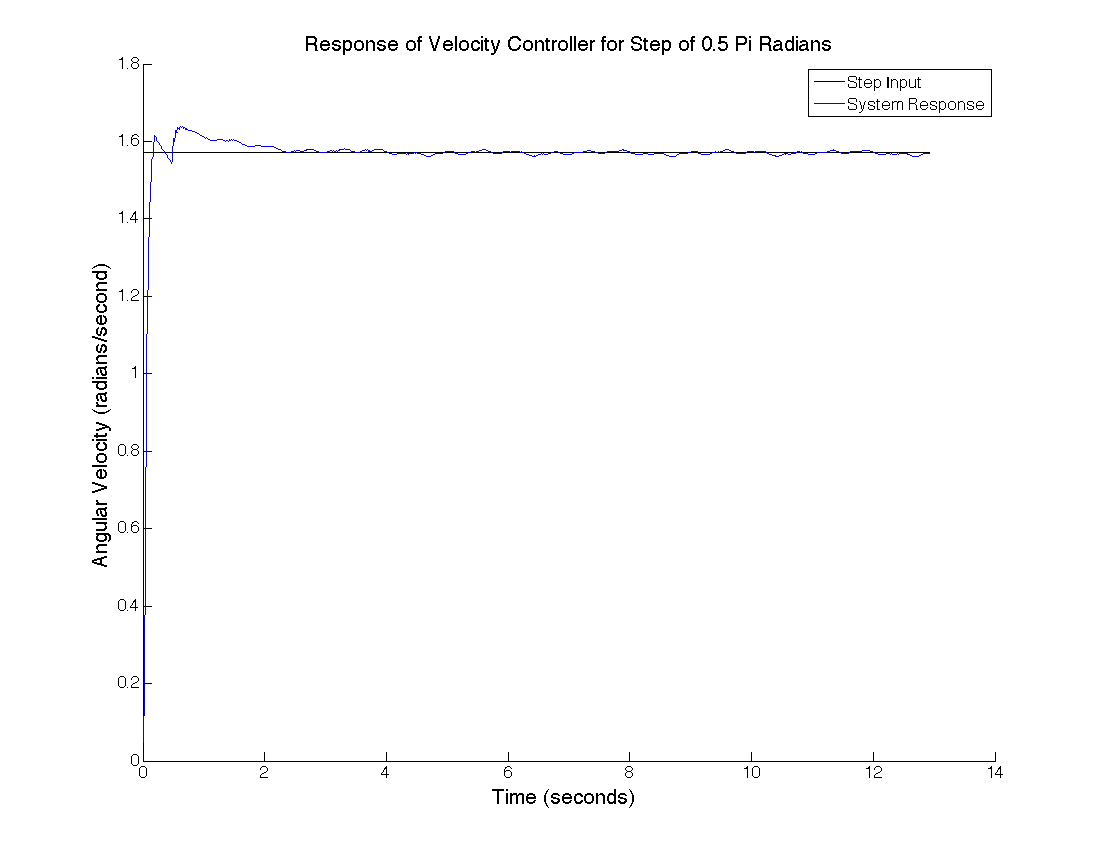
\includegraphics[width = 12cm]{velstep0_5Pi.png}
\caption{Velocity Controller Step Response}
\label{q6_1}
\end{center}
\end{figure}

\begin{figure}[htb]
\begin{center}
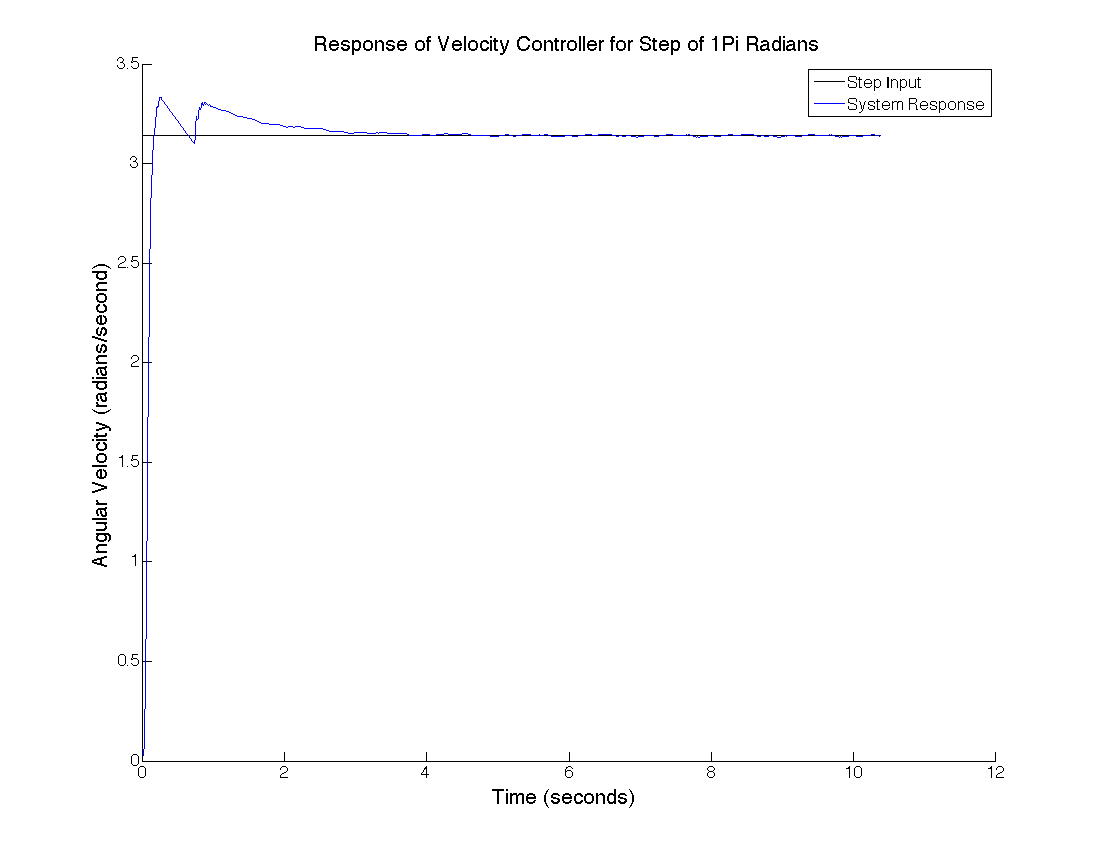
\includegraphics[width = 12cm]{velstepPi.png}
\caption{Velocity Controller Step Response}
\label{q6_2}
\end{center}
\end{figure}

\begin{figure}[htb]
\begin{center}
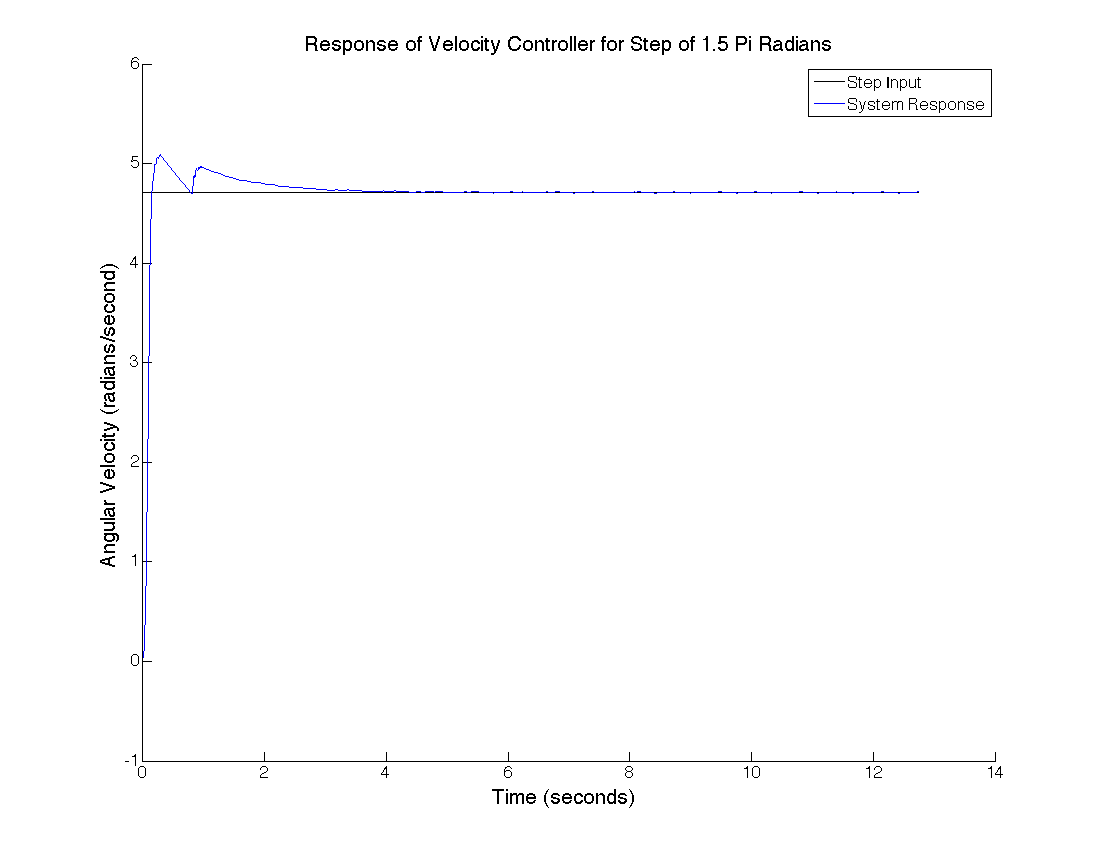
\includegraphics[width = 12cm]{velstep1_5Pi.png}
\caption{Velocity Controller Step Response}
\label{q6_3}
\end{center}
\end{figure}

\begin{figure}[htb]
\begin{center}
\includegraphics[width = 12cm]{velstep5Pi.png}
\caption{Velocity Controller Step Response}
\label{q6_5}
\end{center}
\end{figure}

\begin{figure}[htb]
\begin{center}
\includegraphics[width = 12cm]{velstep10Pi.png}
\caption{Velocity Controller Step Response}
\label{q6_6}
\end{center}
\end{figure}

Figure \ref{q6_7} shows the noise attenuation during a step input of 2$\cdot\pi$ radians/sec. To simulate the noise within LabView, we added a 60 Hz sine signal with an amplitude of 1 to the output of the DAQ assistant, just as with the position controller. Figure \ref{VelNoiseZoom} shows a zoomed in view after the step has taken place. For the step response with no noise, our peak steady state error was 0.010, and with the noise the highest error is 0.20. Given that we were inputting a noise amplitude of one and the error only increased by 0.19, we have attenuated the noise by approximately 5.26 times. This meets the goal of a five times reduction.\\

\xxx{Compare to simulation results}

\begin{figure}[htb]
\begin{center}
\includegraphics[width = 12cm]{velstep2PiwNoise.png}
\caption{Velocity step response for input of 2$\cdot{\pi}$ with a 60 Hz noise signal (amplitude = 1)}
\label{q6_7}
\end{center}
\end{figure}

\begin{figure}[htb]
\begin{center}
\includegraphics[width = 12cm]{VelErrorNoise.png}
\caption{Steady state velocity step response for input of 2$\cdot\pi$ with a 60 Hz noise signal (amplitude = 1)}
\label{VelNoiseZoom}
\end{center}
\end{figure}

\begin{table}[htb]
\begin{center}
    \begin{tabular}{|c|c|c|}
        \hline
        Step Input Amplitude (Radians) & $2 \cdot \pi$ & $2 \cdot \pi$ with Noise \\ \hline
        Rise Time (seconds)            & 0.14          & 0.135                    \\ 
        Settling Time (seconds)        & 1.9700        &  -                    \\ 
        Percent Overshoot (\%)         & 11.3925       & 29.6000                  \\ 
        Steady State Error (\%)        & 0.058328      & 0.054649                 \\
        \hline
    \end{tabular}
\end{center}
\end{table}

The velocity controller we were using for the step response and noise attenuation did not not perform well with sinusoidal inputs, therefore we modified to gains to try to improve the frequency response. The relevant values are given in the table \ref{VelFreqGains}, and the following figures show the response at various frequencies with an amplitude of $\pi$/2. Figure \ref{VelFreqError} shows the error as a function of input frequency. During our tests the velocity output remained stable up to 5 Hz, but the output amplitude error increased greatly. The error exceeded 5\% just beyond 2.2 Hz. This does not meet the goal of less than 5\% error up to 5 Hz.\\

\xxx{Compare to simulation}

\begin{table}[htb]
\begin{center}
    \begin{tabular}{|c|c|c|c|c|}
        \hline
        Gains & P   & I & D     & Filter $\tau$   \\ \hline
        Velocity Loop       & 2   & 9    & 0.3   & 6.5797  \\ 
       \hline
    \end{tabular}
\end{center}
\caption{Values of velocity controller for frequency response}
\label{VelFreqGains}
\end{table}

$$\text{Predicted Bandwidth } =  \xxx{SOMETHING}$$
$$\text{Experimental Bandwidth } =  2.9 Hz$$

\begin{table}[htb]
    \begin{tabular}{|c|c|c|c|c|}
        \hline
        Frequency (Hz) & Input Amplitude & Output Amplitude & Magnitude (dB) & \%Error      \\ \hline
        1              & $\pi/2$         & 1.649            & 0.422015572    & 4.978600463  \\ 
        2              & $\pi/2$         & 1.632143         & 0.332766594    & 3.905450513  \\ 
        2.9            & $\pi/2$         & 1.11778          & -2.955270847   & -28.83991508 \\ 
        3              & $\pi/2$         & 1.06516          & -3.374100561   & -32.18980833 \\ 
        4              & $\pi/2$         & 0.581875         & -8.625803574   & -62.956687   \\ 
        5              & $\pi/2$         & 0.47833          & -10.32784514   & -69.54856643 \\
        \hline
    \end{tabular}
    \caption{Numerical results of velocity control.}
    \label{q6_table}
\end{table}

\begin{figure}[htb]
\begin{center}
\includegraphics[width = 14cm]{VelocityControl_Error.png}
\caption{Velocity error vs. frequency for an input amplitude of $\pi$/2 rad/sec}
\label{VelFreqError}
\end{center}
\end{figure}

To determine the closed-loop bandwidth of the system, we slowly increased the frequency of the input signal until the output amplitude just crossed -3 dB (for a input of $\pi$/2 this corresponded to an output of 1.11), just as we did in section 4 to determine the bandwidth of the position controller. We found that the bandwidth of our position control system was  2.9 Hz, as shown in figure \ref{VelBandwidth}.\\

\begin{figure}[htb]
\begin{center}
\includegraphics[width = 14cm]{VelocityControl_Magnitude.png}
\caption{Output magnitude vs. frequency used to determine bandwidth of velocity controller}
\label{VelBandwidth}
\end{center}
\end{figure}

Just like with the position controller, we faced a lot of trouble meeting all of the performance specifications with just one controller. Again, we found that when we adjusted gains to meet the step requirement, the frequency response usually got worse, and vice-versa. As we mentioned in section 4 ,it's possible that some of the values used in our simulation are incorrect, or that there are other factors we did not account for. In the end we were able to meet the steady state error for step input and noise attenuation requirements, but were not very close to the frequency response requirement.\\

\clearpage

\section*{Appendix : Matlab Code}
\subsection*{enchancedParameterEstimation.m}
\verbatiminput{enchancedParameterEstimation.m}

\subsection*{flatInterpolate.m}
\verbatiminput{flatInterpolate.m}

\subsection*{testParameterEstimation.m}
\verbatiminput{testParameterEstimation.m}


\end{document}